\documentclass[conference]{IEEEtran}
\IEEEoverridecommandlockouts
% The preceding line is only needed to identify funding in the first footnote. If that is unneeded, please comment it out.
\usepackage[left=1.62cm,right=1.62cm,top=1.9cm,bottom=4.4cm]{geometry}
\setlength{\columnsep}{0.25in}
\usepackage{cite}
\usepackage{algorithmic}
\usepackage{graphicx}
\usepackage{textcomp}
\usepackage{xcolor}
\usepackage{natbib}
\usepackage{booktabs}
\usepackage{amsmath,amssymb,amsfonts}
\usepackage{CJK}
\usepackage{CJKutf8}
\usepackage{pinyin}
\bibpunct{[}{]}{;}{a}{,}{,}

% Useful packages
\usepackage{amsmath, amssymb, amsfonts} % Pacotes matemáticos
\usepackage{graphicx} % Inclusão de imagens
\usepackage[colorlinks=true, allcolors=blue]{hyperref} % Links coloridos

% Pacotes para tabelas
\usepackage{booktabs}
\usepackage{multirow}
\usepackage{makecell}
\usepackage{tablefootnote}
\usepackage{threeparttable}
\usepackage{tabularx}



\def\BibTeX{{\rm B\kern-.05em{\sc i\kern-.025em b}\kern-.08em
    T\kern-.1667em\lower.7ex\hbox{E}\kern-.125emX}}
\begin{document}
\begin{CJK*}{UTF8}{gbsn}%{bsmi}

\title{Quantitative Analysis of Translation Quality and Computational Cost in Semantic and Phonetic Translation of Chinese Scientific Terms\\
%Character and Component Threshold Determination in Chinese, Japanese and Korean Hanzi Image Recognition\\

\thanks{This work has been partially supported by the Brazilian National Council for Scientific and Technological Development (CNPq) under the grant number 309545/2021-8.}
}

%Names
\author{\IEEEauthorblockN{Li Weigang, Rafael M. Ramos}
\IEEEauthorblockA{\textit{Computer Science Department} \\
\textit{University of  Brasilia}\\
Brasília, Brazil \\
weigang@unb.br, rafaelmr@gmail.com}
\and
% \IEEEauthorblockN{Li Weigang}
% \IEEEauthorblockA{\textit{Computer Science Department} \\
% \textit{University of  Brasilia}\\
% Brasília, Brazil \\
% weigang@unb.br}
% \and

\IEEEauthorblockN{Pedro C. Brom}
\IEEEauthorblockA{\textit{Math Department} \\
\textit{Federal Institute of Brasilia}\\
Brasília, Brazil \\
pedro.brom@ifb.edu.br}

%\and
%\IEEEauthorblockN{Pedro Carvalho Brom}
%\IEEEauthorblockA{\textit{Computer Science Department} \\
%\textit{University of  Brasilia}\\
%Brasília, Brazil \\
%pcbrom@gmail.com}

}

\maketitle

\begin{abstract}
The representation of scientific terms in Chinese has been a key focus of the scientific community, yet few studies have quantitatively analyzed it from a language model perspective. This paper examines the Chinese naming of the periodic table and organic compounds, exploring the generative properties of Chinese characters and words. By integrating UNICODE/UTF-8 encoding, it compares the representation and computational cost of scientific terms across Chinese, Japanese, Korean, English, Portuguese and Russian. A framework is proposed to evaluate translation quality and computational efficiency for paraphrasing and transliteration in ideographic languages. First, a back-translation method (Chinese → English → Chinese) is used to assess LLMs such as Grok, DeepSeek and ChatGPT. Then, LLMs analyze the impact of semantic and phonetic translation on chemical terms. Results show that Chinese paraphrased naming in the periodic table outperforms Japanese and Korean transliteration-based approaches in accuracy (BLEU: 0.94-0.97) and efficiency (3 bytes per element). In contrast, transliterated Chinese names for certain organic compounds perform poorly (BLEU: 0.16-0.33) and significantly increase byte usage. This study highlights the advantages of leveraging the semantic generative properties of Chinese for scientific terminology, improving comprehensibility and cross-linguistic transferability. It further advocates for semantic translation strategies to enhance term sustainability, accessibility and multimodal advancements in Chinese NLP (CNLP).
\end{abstract}

\begin{IEEEkeywords}
CNLP, Chinese semantic generative, NLP, Semantic and Phonetic Translation, Scientific Terms.
\end{IEEEkeywords}
%修改版引言
\section{INTRODUCTION}

The synergistic advancement of Large Language Models (LLMs) and artificial intelligence has ushered in a paradigm shift in natural language processing (NLP) \citep{vaswani2017attention}. With the breakthrough of Transformer-based architectures, LLMs have demonstrated remarkable capabilities in text generation and cross-lingual translation. Nevertheless, their application to non-English languages—particularly complex systems such as Chinese—continues to pose significant challenges. Among these are the preservation of poetic intent, cultural nuance, and domain-specific terminology \citep{zhang2021study, zhong2024beyond}.

Chinese, spoken by over 1.6 billion people globally \citep{eberhard2023ethnologue}, presents unique difficulties due to its syntactic structure, culturally embedded expressions, and specialized lexicons (e.g., heterocyclic compounds such as “thiazole” and “pyridine”). As such, Chinese–English translation remains one of the most persistent challenges in the development of language intelligence systems \citep{sun2021chinesebert}. Furthermore, Chinese characters exhibit multimodal characteristics traceable to Xu Shen’s Shuowen Jiezi and the ancient Liu Shu (Six Writings), which include ideographic and phonosemantic mechanisms. These provide historical insights into modern LLMs’ grapheme–phoneme joint encoding strategies \citep{weigang2024six}.

Today, Chinese–English and other cross-lingual translation tasks have evolved beyond mere linguistic conversion; they serve as critical infrastructure for globalization, particularly in domains such as international trade, scientific exchange, and cultural transmission. In 2024, China’s foreign trade volume approached USD 6 trillion \footnote{www.chinadaily.com.cn/a/202502/12/WS67abd994a310a2ab06eab9e6.html}, and translation quality directly impacts contract execution, product compliance, and supply chain efficiency. In science, over 25\% of the world's SCI papers in 2023 originated from China, with around 40\% requiring English translation for international publication \citep{jiang2020nsfc}. Conversely, foreign researchers rely on translation to access Chinese advances. In the cultural domain, the 2025 global release of \textit{Nezha: Rebirth of the Demon Child 2} surpassed USD 200 million in North American box office sales \footnote{www.chinadaily.com.cn/a/202503/04/WS67c5d351a310c240449d8511.html}, facilitated by English dubbing and subtitling—demonstrating the necessity of culturally sensitive translation, which traditional tools struggle to achieve.

Despite their excellence in English-centric tasks, LLMs remain limited in Chinese processing due to structural asymmetries between the two languages. Transformer-based models such as ChatGPT are typically pre-trained on word-based English tokens using long-range contextual attention \citep{vaswani2017attention}. This architecture is well-suited to space-delimited languages like English. In contrast, Chinese presents two fundamental challenges \citep{weigang2024threshold}: (1) the lack of explicit word boundaries, making tokenization inherently ambiguous, and (2) the more even distribution of information at the character level, which dominates Chinese tokenization, training, and BLEU-style evaluation \citep{papineni2002bleu}.

However, Chinese linguistic structure is not fully compatible with purely character-based modeling. While most high-frequency units (+-95\%) are one- or two-character words (e.g., “技术” [technology], “翻译” [translation]) \citep{liu1986chinese}, semantically dense three-character terms (e.g., “机器人” [robot]) and four-character expressions (e.g., “人工智能” [AI], idioms like “刻舟求剑”) carry disproportionately high contextual weight. When LLMs treat characters as isolated units, they often fail to preserve the semantic integrity of these word-level expressions, leading to unnatural output or cultural distortion. This explains why LLMs generally perform better on English texts than Chinese, with particularly unstable results in metaphor-rich, poetic, or technical contexts.

Empirical studies confirm this disparity. Mainstream machine translation systems achieve BLEU scores below 0.45 for English-to-Chinese tasks and under 0.27 for Chinese-to-English—substantially lower than scores for other languages such as Russian-to-English (BLEU 43.53) \citep{zhu2025overcoming}. This performance gap is most pronounced in high-stakes domains such as science, law, and medicine. Although hybrid approaches such as sparse Mixture-of-Experts (MoE) models integrated with GPT or LLaMA have shown promise \citep{zhu2025overcoming}, emerging platforms such as CroK, DeepSeek, and Gemini still lack systematic evaluation—particularly in tasks involving cultural nuance, poetic expression, historical references, and scientific nomenclature.

Addressing these limitations requires comprehensive improvements across segmentation strategies, token design, and corpus construction to build a robust Chinese NLP ecosystem. Against this backdrop, this study introduces a Chinese $\rightarrow$ English $\rightarrow$ Chinese back-translation framework as a window to assess the semantic fidelity and cultural retention of LLM outputs \citep{edunov2018understanding,artetxe2018unsupervised}. Specifically, we propose the “Paradox of Poetic Intent” as a conceptual entry point to investigate how LLMs handle linguistic subtlety and cultural meaning in Chinese translation. Figure \ref{fig:imagery_vs_selfawareness} shows the conceptual diagram: The Paradox of Poetic Intent vs. Emergent Quasi-Self-Awareness in LLM verbatim back-translation.

\begin{figure}[htbp]
\centering
\includegraphics[width=0.48\textwidth]{img/BT Image old.png}
\caption{Conceptual Diagram: The Paradox of Poetic Intent vs. Emergent Quasi-Self-Awareness in LLM verbatim back-translation}
\label{fig:imagery_vs_selfawareness}
\end{figure}

It is worth emphasizing that the phenomenon of verbatim back-translation may be interpreted as an internal memory mapping behavior within LLMs. Several recent studies have contributed to our understanding of memory mechanisms in large models. For instance, Brown et al. (2020) \citep{brown2020language} introduced the notion of parametric memory, in which knowledge is implicitly encoded within model weights during training. Shan et al. (2025) \citep{shan2025cognitive} classified LLM memory types from a cognitive perspective; Modarressi et al. (2024)\citep{modarressi2024memllm} proposed structured read-write memory modules to improve long-term retention of rare events;  The Memory framework was developed by Yang et al. (2024) \citep{yang2024memory3} to externalize knowledge, reducing model size and inference cost while maintaining memory capacity; and Zhang et al. (2024) \citep{zhang2024survey} offered a comprehensive survey on memory mechanisms for LLM-based agents.

These works collectively provide theoretical support for understanding verbatim back-translation through the lens of LLM memory. Building on this, we argue that LLMs often exhibit a form of quasi-self-awareness—namely, their spontaneous ability to maintain stylistic and contextual consistency without explicit instruction. Such emergent behaviors may reveal latent context-sensitivity within these models, and open new directions for addressing persistent challenges in NLP, particularly the tension between surface accuracy and deep meaning as posed by the Paradox of Poetic Intent.

To this end, we construct a domain-diverse corpus encompassing three categories: (1) historical translation paradoxes in scientific naming (e.g., the Xue Dejiong dilemma \citep{hejuan2019nomencl}); (2) literary metaphors in cultural texts (e.g., Daolang’s Hua Yao and its spatiotemporal narrative); and (3) idiomatic and terminological expressions drawn from 295 Chinese academic abstracts (CNKI). Using both single-sample and multi-sample experiments, we evaluate six major LLM platforms (e.g., GPT-4.5, Claude 3.7, DeepSeek V3, Grok 3, Gemini 2.0) and three commercial translation tools via a  Chinese $\rightarrow$ English $\rightarrow$ Chinese back-translation paradigm, ensuring statistical significance in our findings.

The main academic contributions of this study are as follows:
\begin{itemize}
\item Establishment of a Chinese back-translation framework combined with multi-sample Friedman testing, used to evaluate the performance of selected language models across four key metrics: BLEU, CHRF, TER, and Semantic Similarity. Results reveal that LLMs perform inconsistently on culturally rich texts, highlighting what we term the “Paradox of Poetic Intent”—a tendency for pretrained models to lose literary depth when striving for literal alignment. Notably, Claude 3.7 and DeepSeek V3 exhibited superior metaphor preservation (average BLEU of 0.60, with a variance of 0.10).

\item Back-translations of scientific abstracts yielded higher adequacy scores than direct translations, suggesting that the iterative process may introduce latent alignment optimization. Meanwhile, traditional translation tools still demonstrate comparative advantages for texts with strong language-specific features—for instance, Sogou Translate achieved a BLEU score of 0.57 on a scientific abstract.

\item LLMs frequently exhibited “verbatim back-translation” effects, especially on platforms like ChatGPT and DeepSeek. This phenomenon, which we describe as a form of “Quasi-self-awareness”, reflects the model's implicit recognition and reconstruction of prior inputs. Such behavior hints at capabilities that transcend traditional translation methods and provides new conceptual ground for advancing LLM-based AGI development.

\item A novel BLEU computation method based on Jieba word segmentation was developed, incorporating Chinese-specific features such as word length, word frequency, and n-gram weighting. This method was contrasted with the currently prevalent character-based BLEU, offering a new perspective for evaluating Chinese translation quality.

\item This study is the first to explicitly propose the concept of the “Paradox of Poetic Intent”—the contradiction wherein an LLM, in seeking literal fidelity during back-translation, sacrifices the depth and nuance of poetic or literary meaning. This insight not only provides a fresh understanding of translation evaluation but also fills a research gap in CNLP regarding the treatment of literary texts such as Huayao. 
\end{itemize}

Overall, this study probes the semantic bottlenecks in Chinese–English translation, offering an objective evaluation of LLMs and commercial translation tools in handling Chinese. The findings serve as a valuable reference for improving bidirectional translation and related CNLP tasks.

%This paper presents five primary academic contributions:
%\begin{itemize}
    
%\item We construct a Chinese back-translation evaluation framework combined with multi-sample Friedman testing, utilizing BLEU, CHRF, TER, and Semantic Similarity as metrics. The results reveal highly inconsistent performance across LLMs when dealing with culturally loaded texts, exposing what we define as the Paradox of Poetic Intent—the tendency of pretrained models to prioritize lexical fidelity while losing deeper literary meaning. Notably, DeepSeek V3 performs best in preserving metaphorical content (BLEU average: 0.60, variance: 0.10).
%\item We find that back-translated scientific abstracts tend to outperform direct translations, suggesting that iterative generation may introduce alignment optimization. Meanwhile, traditional tools still excel in high-domain-specific texts—for example, Sogou Translator achieves a BLEU score of 0.57 on scientific abstracts.
%\item  We identify and analyze a widespread phenomenon of verbatim back-translation, in which LLMs exhibit consistent output patterns across translation cycles, revealing traces of quasi-self-awareness.
%\item  We develop a custom BLEU scoring method based on Jieba word segmentation and n-gram weighting informed by word frequency, providing a new perspective for evaluating Chinese translations beyond character-level tokenization.
%\item We explicitly introduce the concept of the Paradox of Poetic Intent, which describes the inherent tension in LLM-based translation: the pursuit of surface-level alignment often leads to the erosion of poetic or literary essence. This paradox frames both a new lens for translation evaluation and a novel contribution to Chinese NLP research on literary texts such as The Flower Demoness.

%\end{itemize}

%老版引言

\section{INTRODUCTION}

With the rapid advancement of large language models, artificial intelligence has made significant progress in text, image and video generation. When exploring Chinese language models in depth, the generation of Chinese characters and words is recognized as a unique advantage of the Chinese language. As early as nearly two thousand years ago, the classic text Shuowen Jiezi systematically explained the structure of Chinese characters, which holds great significance for modern natural language processing (NLP).

%The Chinese naming of elements in the periodic table exemplifies the natural generative properties and multidimensional information characteristics of Chinese characters. Chinese characters are typically composed of radicals and components. For instance, the combination of radicals such as "钅" (metal), "石" (stone), "气" (gas) and "氵" (water) with other character components naturally forms the single-character names of all 118 chemical elements. This naming method clearly categorizes metals (e.g., 铜, copper), non-metals (e.g., 碘, iodine), gases (e.g., 氧, oxygen) and liquids (e.g., 溴, bromine) in a concise and multimodal manner. Furthermore, these element names serve as roots or affixes for chemical compound names, laying the foundation for the generative structure of Chinese chemical nomenclature.

%\begin{figure}[htbp]
%\centerline{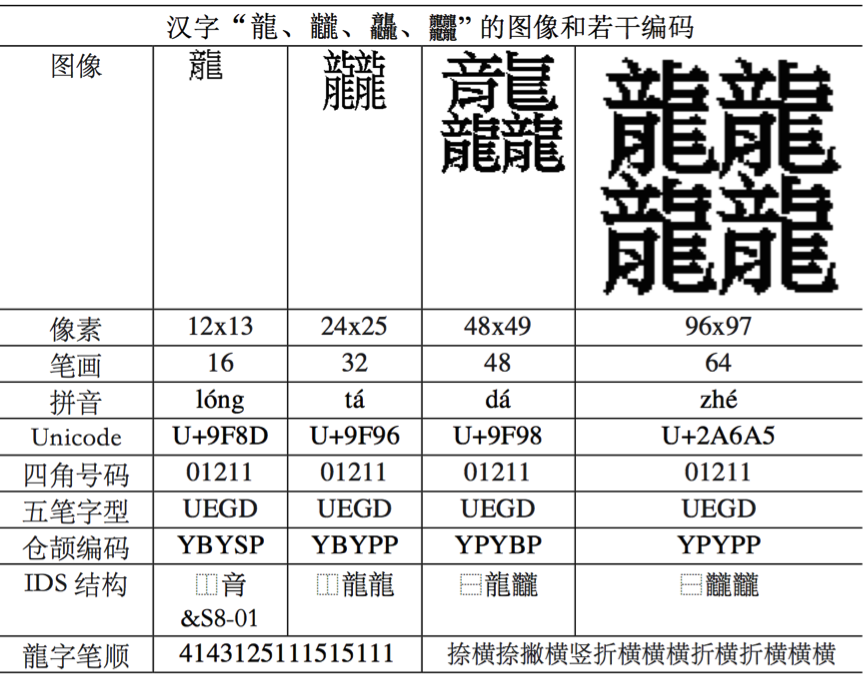
\includegraphics[width = 0.48\textwidth]{Figures/Long 4.png}}
%\caption{A traditional Chinese character "dragon" can be combined into three other Chinese characters, which are two dragons of 32 strokes, three dragons of 48 strokes and four dragons of 64 strokes. These Chinese characters are represented by images of 12, 24, 48 and 96 px.}
%\label{Fig dragon}
%\end{figure}

Among the 118 elements, the longest English element name consists of 13 letters, with an average letter count of 7.82. In contrast, each element's Chinese name requires only a single character, significantly simplifying the presentation of information. Fig. 1 \ref{fig:periodic table compare} illustrates the expression patterns of the same element in both English and Chinese in the "Periodic Table of Chemical Elements." Within squares of the same size, the following information is included: 1) atomic number; 2) element symbol; 3) element name; and 4) atomic weight, among others. However, the uniqueness of Chinese characters allows readers, even those with limited knowledge of chemistry, to infer additional implicit information from a single character. Taking the element "hydrogen" as an example, readers can not only recognize it as a chemical element but also deduce more supplementary information from the character "氢," such as hydrogen being a gas and lighter than air. This ability to compress and add information is a distinct advantage of the Chinese character system.

\begin{figure}[h!]
    \centering
    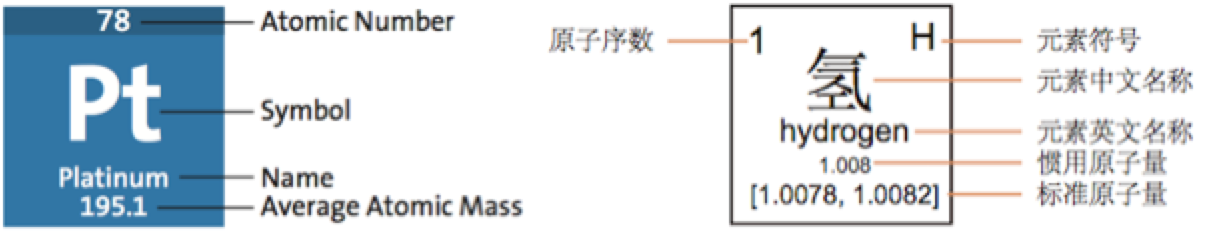
\includegraphics[width = 0.48\textwidth]{img/US and ZH element.png}
    \caption{Example elements from the Periodic Table: platinum (Pt) in the English version and hydrogen (H) in the Chinese version, see Figure \ref{fig:periodic table} in appendix.}
    \label{fig:periodic table compare}
\end{figure}

For a long time, the “Chinese National Committee for Terminology in Science and Technology” has effectively coordinated efforts across various industries in this domain, achieving significant results. However, due to the broad scope of the field and historical legacy issues, certain areas remain less than ideal. For instance, the naming of heterocyclic compounds in Chapter 8: Natural Products of the 《Principles of Organic Compound Nomenclature – 2017》 primarily relies on phonetic transliteration, which differs significantly from the traditional principles used for naming chemical elements and compounds. Moreover, it deviates from the standardized nomenclature revised by the International Union of Pure and Applied Chemistry (IUPAC). 

To illustrate the long-standing debate in the scientific community regarding whether organic compound names should be translated semantically or phonetically, we cite a passage describing this controversy (He, 2019). This case, hereinafter referred to as “Xue Dejiong’s Dilemma”, will serve as a Chinese translation example for further analysis in this study：Xue Dejiong "was dissatisfied with" the simple names using the "mouth radical" (口旁) for "more than ten years," considering them "like the 'Om Mani Padme Hum' in Buddhist scriptures, simply inexplicable!" He argued that if mouth-radical phonetic transliteration characters were used to name heterocyclic compounds like dithiadiazole, it would inevitably result in "something like 'e e thi thi, zole zole zine zine,' filling the page with gibberish, as if it were a foreign text. Even someone as extraordinary as the banished immortal Li Taibai (Li Bai) would likely find it difficult to decipher. Therefore, these simple names with the mouth radical must be abolished (reluctantly abandoned)." Even though he deeply detested the mouth-radical names, he acknowledged that "the structures of fused heterocycles are often complex and intricate, so their systematic names tend to be excessively long. For the sake of convenience in naming and reference, there is indeed a need for specific simplified names." However, he suggested that "based on the sound of the original name, when creating simplified names with mouth-radical characters, at least one additional character should be added at the end to indicate its primary functional group." For example, coffee should be named "caffeine".

%In the field of processing logographic languages such as Chinese, Japanese and Korean (CJK), many scholars have been striving to integrate the mature techniques of phonetic language models to address the unique challenges of logographic language processing. In addition to the development of Chinese LLMs by major information enterprises and the open-source Chinese LLaMA \cite{touvron2023llama,cui2023efficient}, other notable works have emerged. For example, Sun et al. \citep{sun2021chinesebert} proposed the ChineseBERT language model, Zhang et al. \citep{zhang2024hiercode} introduced the HierCode encoding method, Li et al. \cite{li2024drmspell} developed the DRMSpell Chinese spell correction model and Weigang et al.  \cite{weigang2024six} proposed the Six Scripts Multimodal Processing (SWMP) framework. These studies share a common feature of using multimodal techniques to represent the "form, sound and meaning" characteristics of Chinese characters, thus improving the effectiveness of Chinese language processing.

The objective of this study is to leverage language models, particularly large language models (LLMs), to perform machine translation of scientific terms, using translation quality and computational cost as evaluation metrics to quantitatively analyze the differences between semantic translation (paraphrasing) and phonetic translation (transliteration).

Using the Chinese naming conventions of the periodic table and the Principles of Organic Compound Nomenclature – 2017 as case studies, this research explores the natural generative properties of Chinese characters and words. By integrating UNICODE/UTF-8 encoding, it examines differences in representation and processing across Chinese, Japanese, Korean, English, Portuguese and Russian. Based on this, a comparative analysis is conducted to assess semantic vs. phonetic translation strategies in the translation of scientific terminology in ideographic languages. The study highlights the advantages of semantic translation in the Chinese periodic table, demonstrating superior translation accuracy and computational efficiency, while identifying the limitations of phonetic translation in organic compound nomenclature. This underscores the importance of fully utilizing semantic translation strategies in Chinese scientific terminology.

A back-translation approach (Chinese → English → Chinese) is employed to evaluate the translation capabilities of LLMs such as Grok, DeepSeek and ChatGPT. Subsequently, LLMs are used to analyze the effectiveness of semantic and phonetic translation for chemical terminology. The results show that compared to the transliteration-heavy approaches of Japanese and Korean, the semantic naming system of the Chinese periodic table exhibits significant advantages in translation accuracy (BLEU: 0.94-0.97) and computational efficiency (approximately 3 bytes per element). In contrast, phonetic translations of certain organic compounds perform poorly, with BLEU scores ranging from 0.16 to 0.33 and a byte count several times higher, even underperforming Korean transliterations and aligning closely with Japanese results.

These findings demonstrate the importance of quantitatively analyzing semantic and phonetic translation strategies for scientific terminology through language models, offering valuable insights for optimizing Chinese scientific translation. The main academic contributions of this study are as follows:

\begin{itemize}
\item Integration of Historical and Modern Scientific Terminology: a) Reviewing the history of Chinese element naming in the periodic table and analyzing the unique advantages of Chinese characters in scientific terminology. b) Extracting the character formation rules for chemical elements and the naming system for compounds and exploring their applications in natural language processing (NLP).

\item Corpus Collection for Chemical Terminology: a) Using the CNKI (China National Knowledge Infrastructure) Overseas Edition, this study collects scientific literature in eight thematic categories, including artificial intelligence, biotechnology and chemistry. b) Each category consists of around 300 Chinese scientific papers, from which titles, keywords and abstracts are extracted for back-translation analysis. c) In addition, 118 chemical elements and 58 heterocyclic compounds are gathered in multiple languages to serve as a dataset for semantic vs. phonetic translation analysis.
\item Cross-Linguistic Analysis Based on UNICODE/UTF-8 Encoding: a) Proposing a quantitative analysis framework for computational cost comparison between semantic and phonetic translation of scientific terms. b) Evaluating translation cost differences between Chinese, Japanese, Korean and Western languages, highlighting the computational efficiency of Chinese semantic naming.

\item Machine Translation and Quality Evaluation Using Large Language Models (LLMs): a) Establishing a quantitative evaluation method to assess the translation quality of scientific terms in semantic vs. phonetic translation. b) Comparing translation performance across Chinese, Japanese, Korean and Western languages, demonstrating the accuracy advantages of Chinese semantic naming.

\item Advocating for the Use of Semantic Translation in Chinese Scientific Terminology: a) Enhancing the interpretability and cross-lingual transferability of scientific terminology. b) Promoting the generative capabilities of the Chinese language to support advancements in Chinese Natural Language Processing (CNLP), particularly in multimodal generation and intelligent translation applications.
\end{itemize}

\color{blue}
Unlike previous approaches that focus exclusively on translation quality assessment using classic metrics such as BLEU and CHRF, this study proposes a combined analysis of quality and computational cost, considering the efficiency of Unicode/UTF-8 encoding and the impact of phonetic versus semantic translation. Additionally, we integrate a non-parametric statistical framework to validate the observed differences, providing a more robust and quantitative perspective on LLM performance. This approach not only evaluates translation accuracy but also establishes an objective criterion for optimizing scientific nomenclature strategies in Chinese.
\color{black}

\section{Introduction to the Naming of Chinese Chemical Elements and Compounds}
\label{headings}

%Human linguistic abilities are deeply intertwined with cultural backgrounds. The distinction between Americans, French, Brazilians, Chinese and others is often based on their native languages and cultures, which are closely tied to the limits of human cognitive abilities. However, humanoid robots do not face these limitations. Robots possess powerful cross-linguistic capabilities in language processing. They can not only handle multiple languages simultaneously but also switch between different languages instantly according to task requirements. This multilingual processing ability enables humanoid robots to interact with any language user globally, unrestricted by cultural or linguistic boundaries.

Humans are typically proficient in only one or a limited number of languages, which reflect their nationality, culture and identity. In contrast, humanoid robots are not constrained by language barriers. Their multilingual processing capabilities surpass human cognitive limitations, driven by advancements in technology. Robots can rapidly acquire and utilize various languages, thus serving as a bridge across cultural and linguistic divides.

To optimize language resource processing and enhance robotic performance, we examine the Periodic Table and the nomenclature of organic compounds as illustrative examples \citep{wang2010nomencl}. While humans generally read the Periodic Table in their native language, robots must decide which language version to prioritize. By analyzing these cases, we can gain valuable insights into improving robotic efficiency in complex multilingual environments.

%While robots can handle multiple languages, optimizing resource usage and processing efficiency remains a challenge. Balancing resource consumption between different languages is crucial in real-world applications, especially in demanding and time-sensitive environments. Efficient language switching and maintaining processing fluidity require deep optimization of language models. 


%\subsection{The Historical Development of the Chinese Version of the Periodic Table}

%During the late Qing Dynasty, renowned Chinese scientist Xu Shou, in collaboration with British missionary John Fryer, encountered the issue of translating chemical elements, including those in the periodic table, while working on the book The Elements of Chemistry. Xu Shou was the first to propose a systematic approach for naming elements in Chinese characters. His principles included retaining existing Chinese names for elements, adopting reasonable early translations and creating new element names using phono-semantic compounds based on their pronunciation \citep{qiao2022diachronic}. This system brought order to the previously chaotic translation practices and provided standardized language support for subsequent scientific advancements.

%It is said that Xu Shou’s work was inspired by the Zhu Family Genealogy from the Ming Dynasty, which recorded the naming conventions of Zhu Yuanzhang’s descendants. After Zhu Yuanzhang ascended to the throne, he established that the first character of his descendants' names would be predetermined, while the second character would follow the "Five Elements Cycle" (fire, earth, metal, water and wood) as a naming principle. As a result, to avoid name duplications or conflicts with the names of ancestors, many rare Chinese characters appeared in the Zhu family names, some of which later became the names of elements, such as chromium (铬), cobalt (钴) and polonium (钋).

%Although there is no reliable historical evidence to confirm whether Xu Shou was directly inspired by the Zhu Family Genealogy, one thing is clear: the Zhu family’s "Five Elements Cycle" principle greatly enriched the Chinese character system, especially characters related to the five elements. To this day, scientific terminology still benefits from this system.

%Subsequent governments, including the Beiyang Government, the Nationalist Government and several departments of the People's Republic of China, continued to standardize and refine the Chinese version of the periodic table. The Principles of Chemical Nomenclature, published in 1932, established guidelines for naming new elements: names for metallic elements would use the “metal" radical (金) and for non-metallic elements, radicals would reflect the physical state of the element at room temperature: the “stone" radical (石) for solids, the “water" radical (水) for liquids and the “gas" radical (气) for gases. The characters would typically follow a phono-semantic compound structure, with a semantic component on the left and a phonetic component on the right. These naming conventions were widely accepted and promoted within the Chinese cultural sphere, including in Japan and Korea. %Figure \ref{fig:periodic table} in appendix presents the English and Chinese version of the periodic table, produced by the Chinese Chemical Society and the International Union of Pure and Applied Chemistry (IUPAC). \textcolor{blue}{With this standardization in place, the Chinese periodic table today serves as an example of how language can be optimized for processing in multilingual robotic systems.}

\subsection{Advantages of the Chinese Version of the Periodic Table} 

In 1869, Russian chemist Dmitri Mendeleev revolutionized chemistry and atomic science with the periodic table. For phonetic languages like English and Portuguese, translating the periodic table was relatively straightforward. However, adapting it into Chinese presented significant challenges. Early Sino-cultural regions, such as Japan, relied on phonetic transliterations, leading to confusion due to inconsistent usage. Some elements were represented by single characters, while others required multiple characters. %The Chinese periodic table not only addresses these issues of localization but also leverages the unique advantages of Chinese characters. Unlike phonetic symbols, Chinese characters combine form, sound and meaning, transforming element names into phono-semantic compounds that are inherently tied to their properties. %In Figure \ref{fig:periodic table compare}, each element is denoted by a single character alongside its English name. For example, "H" is represented by "氢" (qīng). This character suggests its gaseous state through the radical "气" (qì) while indicating pronunciation with the phonetic component "巠" (qīng), making the representation both compact and information-rich.

The Chinese periodic table not only addresses these issues of localization but also leverages the unique advantages of Chinese characters, which encapsulate visual, phonetic and semantic features. For instance, the element “At" is symbolized by “砹", where the “石" (stone) radical intuitively suggests a non-metal, while “艾" (Ai) provides the phonetic hint. Similarly, “Li" is denoted by “锂", where “钅" indicates metallic properties and “里" contributes the phonetic element. Such phono-semantic combinations simplify the representation and understanding of complex chemical elements, making the Chinese version more efficient for both human learning and machine processing.

Furthermore, the standardized rules for creating new element characters support the generation of symbols for newly discovered elements. For example, on November 30, 2016, the International Union of Pure and Applied Chemistry (IUPAC) announced the English names and symbols for four new elements, completing the seventh period of the periodic table. On May 9, 2017, the Chinese Academy of Sciences, the National Language Committee and the National Science and Technology Terminology Committee jointly released their Chinese names: “钅尔" (nǐ), “镆" (mò), “石田" (tián) and “气奥" (ào).

Figure \ref{fig:four elements} presents examples of four elements (fluorine, neon, chlorine and argon) from the periodic tables of English, Chinese, Japanese and Portuguese. In comparison, the English and Portuguese versions are relatively concise. The Chinese version, however, presents a wealth of information in a more concise and eye-catching manner within the same space. The Japanese version is more complex, with elements represented by either 1-2 kanji characters (e.g., \begin{CJK*}{UTF8}{min}“塩素"\end{CJK*} for chlorine), a combination of kanji and kana (e.g., “弗(フッ)素" for fluorine), or entirely phonetic kana (e.g., “アルゴン" for argon). 
Preliminary statistics indicate that English element names average 7.82 letters in length, which corresponds to 7.82 bytes in Unicode/UTF-8 encoding, with a maximum of 13 letters (and bytes). For Latin language, this average increases slightly to 8.07 letters and bytes, also with a maximum of 13. In contrast, Japanese element names average 4.58 characters in length, occupying approximately 13.73 bytes in Unicode/UTF-8 encoding, with a maximum of 9 characters, taking up to 27 bytes. Additionally, 55\% of the element names exceed the median value of 5 characters. Meanwhile, each Chinese element name is represented by a single character, requiring only 3 bytes in Unicode/UTF-8 encoding making it significantly more concise.

\begin{figure}[h!]
    \centering
    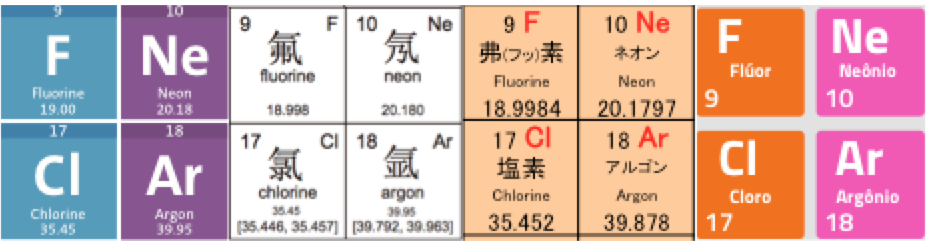
\includegraphics[width = 0.48\textwidth]{img/Four elements.png}
    \caption{Examples of four elements (fluorine, neon, chlorine and argon) from the periodic tables of English, Chinese, Japanese and Portuguese, see Figure \ref{fig:periodic table} in appendix.}
    \label{fig:four elements}
\end{figure}

Chinese scholars insisted on using single Chinese characters, even creating new ones, without resorting to phonetic annotations or pinyin. This practice demonstrates the foresight of Chinese scholars in promoting science popularization and linguistic innovation at that time. This attempt to seamlessly integrate scientific concepts with linguistic symbols remains highly valuable even in today's era of large language models.

Chinese element symbols go beyond being mere chemical representations; they embody a unique cultural phenomenon. By skillfully integrating the phonetic and semantic characteristics of Chinese characters with scientific concepts, they vividly illustrate the depth and versatility of the language. This method of translating abstract scientific ideas into tangible symbols not only aids in research and education but also adds new layers of meaning to Chinese culture. Due to the compactness of Chinese characters, information can be expressed with greater efficiency, reducing cognitive load and enhancing machine processing capabilities. In particular, the phonosemantic structure of Chinese characters optimizes encoding, making computational processing more efficient. This fusion of science and the humanities has created a valuable cultural legacy for future generations.
 
%For robots with cross-linguistic capabilities, the information density of Chinese characters provides an advantage in language processing. When reading the Periodic Table of Elements, the robot can first identify the elements represented by Chinese characters and use their phonosemantic features to quickly generate corresponding multilingual outputs. This processing method not only enhances data compression efficiency but also allows robots to complete complex tasks with lower resource consumption during multilingual interactions.

\subsection{Generating Compound Names Based on Affix and Root Characters}

The naming of Chinese chemical element symbols marks only the beginning of a great endeavor. On this foundation, the naming of organic and inorganic chemical compounds unfolds its vast potential \citep{wang2010nomencl}. The Chinese Chemical Society introduced the “Nomenclature of Organic Compounds-2017," \citep{ccs2017nomenclature} establishing principles such as systematization, standardization, simplification and consistency, which have fostered the orderly and scientific development of chemical research and education  \citep{maning2019ex}.

The naming of organic compounds in Chinese is far more intricate than that of elements or inorganic compounds. Prior to the 20th century, organic compound names were phonetically transliterated from Western languages, leading to cumbersome terms \citep{hejuan2016nomencl}. To resolve this, chemists introduced single-character names like “烷” (alkane), “烯” (alkene) and “炔” (alkyne) based on semantic translation. These concise terms convey the core meaning of the compounds and lay the groundwork for naming their derivatives. For example, the Chinese character for “烃” (hydrocarbon) integrates elements from “碳" (carbon) and “氢" (hydrogen), with a “火" radical symbolizing combustion. Hydrocarbons, made of carbon and hydrogen, are the basis for many organic compounds such as alkanes, alkenes and alkynes. The IUPAC nomenclature system \citep{favre2014nomenclature} is often applied, with single bonds indicating alkanes, double bonds for alkenes and triple bonds for alkynes. Cyclic structures are named as cycloalkanes and those with benzene rings as aromatic hydrocarbons \citep{hejuan2016nomencl}. This alignment with chemical “semantics" demonstrates the evolution from element names to more complex compound terms. %Additionally, root words such as alcohol (醇), aldehyde (醛), ketone (酮), ether (醚) and ester (酯) were created, forming the foundation for the systematic naming of organic compounds in Chinese.

In discussing word formation, prefixes, suffixes, connectors and roots in Chinese compound words are crucial. The “Nomenclature of Organic Compounds-2017" provides detailed naming rules for organic compounds, which cannot be fully covered here. However, the use of Chinese numerals and ordinal terms like the Heavenly Stems gives an insight into this system. %For example, the Heavenly Stems 甲 (jia), 乙 (yi), 丙 (bing), 丁 (ding), 戊 (wu), 己 (ji), 庚 (geng), 辛 (xin), 壬 (ren), 癸 (gui) indicate the number of carbon (or silicon, nitrogen, boron, etc.) atoms in chains or rings of fewer than ten atoms, while higher numbers are represented by standard Chinese numerals. Similarly, 
The terms like “伯" (primary), “仲" (secondary), “叔" (tertiary) and “季" (quaternary) denote the substitution level of hydrogen atoms in hydrides. For example, hydrocarbons have primary, secondary, tertiary and quaternary carbons, while amines correspond to primary, secondary, tertiary amines and quaternary ammonium salts. These terms parallel their English counterparts and align Chinese and English naming conventions \citep{ccs2017nomenclature}.

The Chinese character element symbols go beyond simple chemical notation and represent a cultural phenomenon, creatively merging phonetic and semantic elements with scientific knowledge. This method makes complex scientific ideas more tangible and supports research and education, while also enriching the cultural heritage of Chinese characters. Moreover, applying Chinese characters in chemical nomenclature, especially in constructing compound words, offers valuable insights for CNLP. This is a key point of this article. The efficiency of Chinese characters in expressing information reduces computational complexity, making language models more effective. 

\subsection{Quantitative Analysis of Semantic and Phonetic Translation in Modern Scientific Terminology Using LLMs}
The Chinese version of the Periodic Table of Elements and the naming conventions for organic compounds can be regarded as exemplary models of the integration of science and technology with linguistic artistry. As mentioned earlier, the Principles of Organic Compound Nomenclature issued by the Chinese Chemical Society in 2017, with its principles of systematization, standardization, simplification and consistency, has provided a scientific foundation for the orderly development of chemical research and education (Ma Ning et al., 2019). Its concepts, methods, rules and implementation capabilities have set an example for other industries, even forming a cultural heritage with far-reaching influence. In the era of large language models, these achievements directly benefit from such efforts.

However, the Principles of Organic Compound Nomenclature-2017 also contains some inconsistencies, particularly in the naming of heterocyclic compounds, which primarily adopts a phonetic translation approach. According to historical records, the Chemical Nomenclature Principles promulgated by the Ministry of Education of the Republic of China in 1932 established a unified standard for Chinese chemical terminology. For basic heterocyclic parent structures, it introduced phonetic translations using "two characters with the mouth radical (口)" as simplified names. In the early years of the People's Republic of China, many chemists expressed dissatisfaction with these mouth-radical simplified names. They proposed creating ideographic Chinese characters to denote heterocyclic parent structures, combined with the names of heteroatoms, to form systematic names for heterocyclic compounds. The Principles issued in 1950, 1953 and 1960 adopted this ideographic approach for systematic names of heterocyclic parent structures but did not abolish the mouth-radical simplified names. The 1980 Principles rejected the previous ideographic names for heterocycles and re-established the mouth-radical phonetic names, which have been used ever since (He Juan, 2019). This issue is vividly reflected in the aforementioned "Xue Dejiong's Dilemma."

At the time, there was a lack of quantitative analysis methods to study the differences between semantic and phonetic translations in the naming of heterocyclic compounds, preventing a deeper exploration of the issue. However, with the widespread application of large language models today, such quantitative analysis has become possible. This paper employs artificial intelligence methods to conduct a quantitative analysis of the naming of scientific terminology, while drawing on the experience of Chinese character generation in chemical element naming to advance research on Chinese language models.

\section{Quantitative Analysis of Multilingual Chemical Element and Compound Naming}
This section constructs a general corpus based on Chinese literature information from the China National Knowledge Infrastructure (CNKI) Overseas Edition, the Periodic Table and multilingual naming data of heterocyclic compounds. By analyzing the Unicode/UTF-8 encoding methods of relevant languages, this study quantitatively researches the computational cost of chemical substance naming across different languages.

\subsection{Basic Corpus}

\subsubsection{Periodic Table Corpus}

This study constructs an element name corpus based on the multilingual element names of the Periodic Table. This corpus includes element names in six languages: English (EN118), Russian (RU118), Portuguese (PT118), Latin (LA118), Chinese (ZH118), Japanese (JA118) and Korean (KO118). Among these, English, Russian, Portuguese and Latin are phonetic languages. Korean element names are direct phonetic transcriptions from English. Chinese element names are ideographic translations from English and are further divided into three versions based on regional differences: Simplified Chinese for mainland China (ZH-CN118), Traditional Chinese for Taiwan (ZH-TW118) and Traditional Chinese for Hong Kong (ZH-HK118). Japanese element names are more complex, combining three forms: Kanji (ideographic), Kanji and Kana (ideographic + phonetic) and pure Kana (phonetic). Therefore, this study collected a total of eight Periodic Table corpora.

\subsubsection{Corpus from the Principles of Organic Compound Nomenclature}
The Principles of Organic Compound Nomenclature-2017 states that the nomenclature of Chinese organic compounds mainly includes three methods: ideographic translation, phonetic transcription and common usage of English names. When the compound name is relatively complex, a combination of these three methods can also be used. Chapter 8, 'Natural Products,' in the catalog of the Principles is significantly different from other chapters: firstly, the listed compound names are mostly phonetic transcriptions in Chinese characters; secondly, almost every name is followed by its original English name, as shown in Figure 3. Therefore, this study selected 58 organic compound names from this chapter to construct two corpora, Simplified Chinese (ZH58) and English (EN58), which serve as typical corpora for Chinese phonetic transcriptions of organic compound names. It can be seen that without English assistance, these Chinese compound names are difficult to understand and memorize. Another drawback of Chinese phonetic transcriptions of compounds is the weak regularity of nomenclature. For example, in the term 'bisbenzyltetrahydroisoquinolines,' there is the ideographically translated character '氢' (hydrogen) and the phonetically transcribed '喹啉' (quinolines). This brings difficulties to Chinese-English name translation. However, these analyses are not the focus of this study. In the following chapters, we will mainly focus on two aspects: the computational cost of language processing and the effectiveness of language processing, such as translation accuracy.

\subsubsection{Scientific and technical literature corpus}

This study retrieves relevant journal literature information from the China National Knowledge Infrastructure (CNKI) Overseas Edition (oversea.cnki.net), including journal names, paper titles, authors, keywords, abstracts, volume numbers and page numbers. Based on ten topics, including chemistry, biotechnology, nanotechnology, telemedicine, artificial intelligence, data science, digital economy, linguistics, sociology and distance education, 295 Chinese scientific literature titles, keywords and abstracts were collected for each topic to construct a general corpus and uploaded to GitHub. The order of the above disciplines is basically arranged according to the difficulty of language processing. This ensures that in the subsequent 'Chinese-English-Chinese' reverse translation and other language processing, the sample size for each category reaches 295, making the analysis results statistically significant.

For example: Sun Liping, Tong Zilong, Qian Qian, Lu Xintao, Ling Chen, Fang Cheng, Tang Qiyu, Jiang Xiao. (2024). Two-Stage Fine-Tuning of Professional-Level Large Language Models Based on Medical Clinical Data. Computer Applications Research, 41(10), 2906-2910.

\subsection{Statistical Analysis of Computational Cost for Language Processing}
For Chinese nomenclature of chemical terms (such as element names and organic compound names), two methods are commonly used: ideographic translation and phonetic transcription. This study will quantitatively analyze the ideographic and phonetic transcription effects of chemical terms based on the Unicode/UTF-8 encoding system. If fewer bytes are required for encoding, it indicates that the term nomenclature is scientific and the language processing effect is good; conversely, it indicates that the nomenclature effect is poor and should be avoided as much as possible.

For the convenience of comparative analysis, using English representation as the baseline, the ratio γ (gamma) of the representation of element or compound nomenclature in a certain language to the English representation is defined as following.

If the representation number is the number of characters $N_{L,\text{char}}$, then $\gamma$ is the character ratio relative to English:
\begin{equation}
\gamma_{\text{char}} = \frac{N_{L,\text{char}}}{N_{\text{Eng},\text{char}}}
\label{eq:char_ratio}
\end{equation}

If the representation number is the number of bytes $N_{L,\text{byte}}$, then $\gamma$ is the byte ratio relative to English:
\begin{equation}
\gamma_{\text{byte}} = \frac{N_{L,\text{byte}}}{N_{\text{Eng},\text{byte}}}
\label{eq:byte_ratio}
\end{equation}

\subsubsection{Comparative Analysis of Multilingual Nomenclature in the Periodic Table}
Statistical data in Table \ref{tab:letter_byte_comparison} shows that the average length of 118 English names in the Periodic Table is 7.82 letters, equivalent to 7.82 bytes in Unicode/UTF-8 encoding, with the longest being 13 letters (bytes). For Latin, the average length slightly increases to 8.07 letters and bytes, with the maximum length still being 13 letters. In contrast, Japanese element names average 4.58 characters, occupying approximately 13.73 bytes in Unicode/UTF-8 encoding, with a maximum of 9 characters, occupying 27 bytes. Additionally, among the 118 elements, 55\% of the element names exceed the median length of 5 characters. In comparison, each Chinese element name is represented by only one character, requiring only 3 bytes in Unicode/UTF-8 encoding, while the average number of bytes for Japanese element names is 4.58 times that of Chinese.

\begin{table*}[h!]
\centering
\caption{Comparison of Representation Indicators for Periodic Table Names in Several Languages}
\begin{tabular}{|c|c|c|c|c|c|}
\hline
 & \textbf{Minimum letters} & \textbf{Maximum letters} & \textbf{Average letters} & \textbf{Average bytes} & \textbf{Byte ratio} \\ 
 & \textbf{最少字符} & \textbf{最多字符} & \textbf{平均字符} & \textbf{平均字节(UTF-8)} & \textbf{字节比} \\ \hline
\textbf{English 英文} & 3 & 13 & 7.82 & 7.82 & 1 \\ \hline
\textbf{Latin 拉丁文} & 4 & 13 & 8.07 & 8.07 & 1.05 \\ \hline
\textbf{Portuguese 葡萄牙文} & 4 & 12 & 7.05 & 7.27 & 0.96 \\ \hline
\textbf{Russian 俄文} & 3 & 11 & 6.66 & 13.32 & 1.70 \\ \hline
\textbf{Japanese 日文} & 1 & 9 & 4.58 & 13.73 & 1.76 \\ \hline
\textbf{Korean 韩文} & 1 & 8 & 2.99 & 8.97 & 1.15 \\ \hline
\textbf{Chinese 中文} & 1 & 1 & 1 & 3 & 0.38 \\ \hline
\textbf{SWPC} & 4 & 8 & 4.75 & 4.75 & 0.61 \\ \hline
\end{tabular}
\label{tab:letter_byte_comparison}
\end{table*}

Furthermore, the Korean Periodic Table nomenclature comprehensively adopts phonetic transcription, similar to Japanese Kana nomenclature, rather than ideographic translation (like Kanji). Most element names are based on the Korean transcription of their English or Latin pronunciations, rather than Chinese-style translations based on chemical properties. However, due to historical and habitual usage reasons, a few common elements retain Chinese pronunciations. Additionally, 12 elements are directly represented by English letters. These 12 elements have been excluded from the statistics in Table \ref{tab:letter_byte_comparison}. Korean element names average 2.99 characters, occupying approximately 8.97 bytes in Unicode/UTF-8 encoding, which is about 3 times that of Chinese; and the longest element name is 8 characters, occupying 24 bytes.

To briefly summarize, the relevant data for the Periodic Table are as follows: the character ratio for Chinese element names is 0.1278 and the byte ratio is 0.3835; the character ratio for Japanese is 0.5850 and the byte ratio is 1.7551; the character ratio for Korean is 0.3824 and the byte ratio is 1.1473. From the perspective of language processing computational cost, the representation of Chinese ideographic element names is far superior to that of Japanese and Korean names based on phonetic transcription.

\subsubsection{Comparative Analysis of Multilingual Compound Nomenclature in Phonetic Transcription} 
As described in the basic corpus above, the Simplified Chinese ZH58 corpus and the English EN58 corpus both consist of 58 phonetically transcribed Chinese organic compound names. This study translates the corresponding Japanese JA58 corpus and Korean KO58 corpus based on the EN58 corpus. Table \ref{tab:comparison} presents a comparison of the representation indicators for several languages' phonetically transcribed organic compound names.

\begin{table*}[htbp]
\centering
\caption{Comparison of Representation Indicators for Phonetically Transcribed Organic Compound Names}
\label{tab:comparison}
\begin{tabular}{|c|c|c|c|c|c|}
\hline
\textbf{Language} & \textbf{Minimum letters} & \textbf{Maximum letters} & \textbf{Average letters} & \textbf{Average bytes} & \textbf{Byte ratio} \\
\textbf{语言} & \textbf{最少字符} & \textbf{最多字符} & \textbf{平均字符} & \textbf{平均字节(UTF-8)} & \textbf{英语字节比} \\
\hline
English 英文 & 9 & 35 & 13.67 & 13.67 & 1 \\
\hline
Japanese 日文 & 4 & 18 & 6.43 & 19.34 & 1.41 \\
\hline
Korean 韩文 & 2 & 17 & 5.05 & 15.16 & 1.11 \\
\hline
Chinese 中文 & 3 & 12 & 6 & 18 & 1.30 \\
\hline
\end{tabular}
\end{table*}

From Table \ref{tab:comparison}, it can be observed that in the Chinese transliterations of heterocyclic organic compound names, the character ratio is 0.4388 and the byte ratio is 1.3165. For Japanese, the character ratio is 0.4716 and the byte ratio is 1.4149. For Korean, the character ratio is 0.3695 and the byte ratio is 1.1084.

In the case of transliterated compounds, the byte representation of Chinese is close to that of Japanese and both are higher than Korean transliterations. This essentially eliminates the advantages of semantic naming in the periodic table, which is a key strength of Chinese element nomenclature. These findings indicate that the Chinese transliteration strategy for heterocyclic compounds is suboptimal and from the perspective of computational efficiency in language processing, it performs significantly worse than the semantic naming approach in Table \ref{tab:letter_byte_comparison}.

\section{Translation Performance for Semantic and Phonetic Translation of Chemical Elements and Compounds}
The technical approach of this section is as follows: 1) Back Translation Technique: Utilize scientific literature corpora to evaluate the machine translation performance of language models, particularly large language models (LLMs). 2) Cross-Language Translation Analysis: Based on the above, employ language models to analyze the effectiveness of multilingual translation, using corpora of chemically named entities semantic translation for chemical elements and phonetic translation for heterocyclic compounds. This approach aims to compare the effectiveness of semantic and phonetic translation.

The underlying assumption is that if machine translation performs well, the corresponding translation mode whether semantic or phonetic should also be effective.

\subsection{Evaluation of Machine Translation Performance}
The main methods for evaluating machine translation performance include the following:
\begin{itemize}
   
 \item Reference-based Evaluation: Experts or LLMs (Large Language Models) act as reviewers, comparing the source text, machine-translated text and reference translations. They provide objective scores or calculate relevant evaluation metrics based on criteria such as fluency, accuracy and fidelity.

 \item Reference-free Evaluation: In the absence of human reference translations, experts or LLMs directly assess the reasonableness of machine translations by: a) Generating multiple possible translations and evaluating whether the machine-translated text is appropriate. b) Leveraging the knowledge and reasoning capabilities of LLMs to determine if the translation aligns with the context. c) Using back-translation to check if the translated text can be restored to the original text.

 \item Machine Translation Evaluation Metrics: BLEU (Bilingual Evaluation Understudy) is a common metric for assessing the quality of machine translation. It measures the similarity between automatically translated text and human reference translations. The core idea is to calculate the matching degree of n-grams to evaluate the fluency and accuracy of the translation.

\end{itemize}

\subsection{Back-Translation Validation of Translation Performance for LLMs and Translation Tools}
This section employs a back-translation method to translate "Xue Dejiong’s Dilemma”." This Chinese text encompasses chemical terminology (e.g., oxothiazine, zolozazine), religious colloquialisms (e.g., "Om Mani Padme Hum"), cultural allusions (e.g., "Li Taibai, the Banished Immortal"), a distinctive rhetorical style and rich emotional expression. Even for native Chinese speakers without a university-level education, fully comprehending the text poses a significant challenge. This complexity makes it an effective test case for evaluating the Chinese comprehension and translation capabilities of language models. Two categories of language models are primarily selected: 1) widely used translation tools, such as Google Translate, Baidu Translate and Sogou Translate; and 2) prevalent large language models (LLMs), including ChatGPT, Grok, DeepSeek and Gemini. These models or tools are publicly accessible systems on the internet, allowing any user to replicate the computations.

This study aims to assess the translation quality of eight language models/tools when handling intricate Chinese texts. The experiment involves translating the original text of "Xue Dejiong’s Dilemma" into English, then back-translating it from English to Chinese and comparing the result with the original text. BLEU scores are calculated to quantify translation accuracy and fidelity, with a particular focus on comparing the performance differences between large language models (LLMs) and traditional translation tools.

Table \ref{tab:bleu_comparison} presents the BLEU scores of the back-translated texts for each model along with a brief evaluation. The BLEU scores were computed using the Grok xAI platform. Specifically, BLEU 1 was calculated based on the translation results of "Xue Dejiong’s Dilemma”" from various platforms on March 7-8, 2025, while BLEU 2 was derived from the translation results of "Xue Dejiong’s Dilemma" along with an additional segment of the original text on March 13-14, 2025.

\begin{table}[h]
\centering
\caption{Comparison of BLEU Scores Across Two Rounds} %for Different Translation Tools}
\label{tab:bleu_comparison}
\begin{tabular}{lccc}
\toprule
\textbf{LLM/Tool}         & \textbf{BLEU 1 (R 1)} & \textbf{BLEU 2 (R 2)} & \textbf{Change} \\
\midrule
Grok (xAI)               & 0.65                     & 0.61                     & -0.04          \\
DeepSeek R1              & 0.64                     & 0.58                     & -0.06          \\
ChatGPT 4.5              & 0.59                     & 0.59                        & 0              \\
ChatGPT 4                & 0.47                     & 0.50                     & +0.03          \\
Gemini Flash 2.0         & 0.51                        & 0.52                     & +0.01              \\
Google Translation       & 0.33                     & 0.44                     & +0.11          \\
Baidu Translation        & 0.25                     & 0.36                     & +0.11          \\
Mistral                  & 0.24                     & 0.46                     & +0.22          \\
Sogou Translation        & 0.17                     & 0.31                     & +0.14          \\
\bottomrule
\end{tabular}
\end{table}

Based on the analysis of the first-round BLEU calculation results in Table \ref{tab:bleu_comparison}, the following preliminary conclusions can be drawn:
\begin{itemize}
 \item Large language models (LLMs) demonstrate outstanding performance in translating complex texts, achieving results comparable to human translation. Grok, DeepSeek and ChatGPT-4.5 ranked among the top three, highlighting the advantages of LLMs in handling complex translation tasks. Notably, ChatGPT-4.5 shows a significant improvement over ChatGPT-4 (0.59 vs. 0.47).
 \item Traditional translation tools, which rely on conventional language models, still exhibit limitations in translating complex texts. Except for Google Translate, which achieved a BLEU score of 0.33, both Baidu Translate (0.25) and Sogou Translate (0.17) had BLEU scores below 0.30. According to the current state-of-the-art (SOTA) in machine translation, BLEU scores for Chinese-to-English translations are generally below 0.45, while those for English-to-Chinese translations are typically below 0.28 (Zhu et al., 2025). This suggests that among conventional language models, Google Translate performs relatively well, whereas Baidu Translate and Sogou Translate still face considerable challenges in handling Chinese texts involving cultural references and specialized terminology, requiring further optimization and improvement. 
\end{itemize}

\subsection{Using LLM Translation to Examine Translation Strategies}
As discussed in Section 2, the translation strategy for scientific terms directly affects their applicability and has a profound impact on the development of specialized fields. Building on the verification of the effectiveness and quality of reverse translation using large language models (LLMs), this section evaluates translated texts generated by LLMs using both semantic translation and phonetic translation strategies. By assessing translation quality, we explore how different translation strategies influence the naming of scientific terms.

\subsubsection{Evaluating the Linguistic Processing of Literal Translation in Element Naming vs. Transliteration in Compound Naming through Reverse Translation}
To analyze the differences between literal translation and transliteration, we designed a Chinese-English-Chinese reverse translation framework: Chinese (LLM1) → English (LLM2) → Chinese, followed by quality assessment using LLM3, where BLEU scores were calculated.

For this experiment, we selected two distinct datasets: 1) ZH100: A dataset containing the Chinese names of the first 100 chemical elements, translated using a literal translation approach. 2) ZH58: A dataset containing the Chinese names of 58 heterocyclic compounds, translated using a transliteration approach.

\begin{itemize}
\item ZH100 back-Translation results: Using DeepSeek, Chinese element names were translated into English, then GPT-4 back-translated them into Chinese and finally, Grok calculated the BLEU score between the original and back-translated Chinese text. The result was 1.00.
\item ZH58 back-Translation results:
1) Using DeepSeek, Chinese compound names were translated into English, then GPT-4 back-translated them into Chinese and Grok calculated the BLEU score. The result was 0.55.
2) Using DeepSeek, Chinese compound names were translated into English, then Gemini back-translated them into Chinese and Grok calculated the BLEU score. The result was 0.65.
\end{itemize}

From a translation quality perspective, the reverse translation of Chinese chemical element names (literal translation) achieved exceptional consistency, with a BLEU score of 1.00, indicating near-perfect linguistic alignment. For instance, “氢” → “Hydrogen” (DeepSeek) → “氢” (GPT-4), demonstrating a lossless transformation. This suggests that the pictophonetic and semantic translation strategy used in chemical element naming has historical significance. Even with modern large language models, this translation method remains highly effective.

In contrast, the reverse translation of heterocyclic compound names (transliteration) yielded significantly lower BLEU scores. For example:
\begin{itemize}  
\item “千里光碱类” → “Senecionines” (DeepSeek) → “千里光宁类” (Gemini), BLEU 0.65
\item “白坚木碱类” → “Aristolochic Acids” (DeepSeek) → “马兜铃内酯类” (GPT-4), BLEU 0.55
\end{itemize}

These results highlight the irreversibility of transliteration in reverse translation, as phonetic variations and structural complexity lead to a significant decline in translation quality. This adds an additional layer of difficulty to language processing when transliteration is involved.

During early testing, we observed an interesting phenomenon: when the same LLM (e.g., DeepSeek or Mistral) was used for both translation and back-translation, the model sometimes produced artificially high BLEU scores due to a "verbatim back-translation" effect. In some cases, the model returned text nearly identical to the original input, regardless of linguistic differences. For example, DeepSeek initially produced a BLEU score of 0.996 for back-translation, an unrealistic result, given that its Chinese-to-English BLEU score was only 0.86.

%Additionally, Gemini refused to process ZH100 due to the complexity and volume of the task, illustrating how different LLMs handle large-scale translation tasks differently.

To mitigate these issues and ensure translation authenticity, we adopted a multi-LLM collaborative approach: 1) LLM1 (DeepSeek) handled the initial translation. 2) LLM2 (GPT-4) performed the back-translation. 3) LLM3 (Grok) evaluated translation quality. This design effectively ensured a more reliable and unbiased assessment of translation strategies.

\subsubsection{Evaluating the Language Processing Performance of Literal Translation and Transliteration Using Machine Translation Tools}
Since Google Translate is one of the most widely used machine translation tools available online, this section first employs Google Translate to translate chemical element names (ZH100 and EN100 corpora) as a representative of the literal translation strategy and heterocyclic compound names (ZH58 and EN58 corpora) as a representative of the transliteration strategy. Additionally, considering the differences between Chinese, Japanese and Korean in representing chemical elements and heterocyclic compounds, we extend the translation experiments to Japanese and Korean to observe how different linguistic systems handle these two strategies.

To objectively assess translation quality, Grok and TILDE (tilde.ai/interactive-bleu) are used to compute BLEU scores, quantifying the accuracy of different translation approaches. Table 5 presents the relevant results.
The experiment covers the following four translation modes: ZH → EN: Translating Chinese into English and comparing it with the original English text; EN → ZH: Translating English into Chinese and comparing it with the original Chinese text; ZH → JA: Translating Chinese into Japanese and comparing it with English-to-Japanese translations; ZH → KO: Translating Chinese into Korean and comparing it with English-to-Korean translations.

Using BLEU scores as the evaluation metric, the results further validate the conclusions drawn from Table 4, while also highlighting differences in the performance of various translation strategies in multilingual environments:
\begin{itemize}
    
\item Chemical element names (following a literal translation strategy) achieve BLEU scores between 0.94 and 0.99 across all four translation modes, indicating that the use of a literal translation approach ensures high stability and consistency in machine translation. In contrast, heterocyclic compound names (following a transliteration strategy) achieve significantly lower BLEU scores (ranging from 0.16 to 0.36), demonstrating that transliteration poses greater challenges for machine translation, particularly when handling complex domain-specific terminology. Even with certain optimizations in Google Translate, the quality of transliterated terms remains difficult to improve significantly.

\item In Chinese-Japanese-Korean (CJK) translation modes, chemical element names maintain high BLEU scores (0.94–0.99), with Chinese-English translation achieving the highest BLEU score (98.73, computed by TILDE). However, for heterocyclic compound names, which rely on transliteration in all three languages, translation quality varies significantly:
\begin{itemize}
    
\item The BLEU score for Chinese ↔ English is the lowest (26.93), reflecting the linguistic processing challenges posed by the transliteration of Chinese heterocyclic compound names, which leads to poor machine translation performance
\item Chinese ↔ Japanese achieves a higher BLEU score (36.28), suggesting that Japanese may have a comparative advantage in processing transliterated Chinese terms.
\item Chinese ↔ Korean achieves a BLEU score of 29.93, ranking between Chinese-English and Chinese-Japanese translations, indicating a certain degree of stability in transliteration processing for Korean. 
\end{itemize}
\end{itemize}
In summary, this experiment further confirms that literal translation strategies provide greater stability in cross-linguistic machine translation, while transliteration strategies suffer from quality degradation due to pronunciation variations and linguistic structure differences. These findings have important implications for the standardization of scientific terminology, the optimization of machine translation systems and NLP terminology processing.

\begin{table*}[htbp]
\centering
\caption{BLEU Scores for Different Translation Modes}
\label{tab:bleu_translation_modes}
\begin{tabular}{|c|c|c|c|c|c|c|c|c|}
\hline
\textbf{Translation Mode} & \multicolumn{2}{c|}{\textbf{Chinese → English}} & \multicolumn{2}{c|}{\textbf{English → Chinese}} & \multicolumn{2}{c|}{\textbf{Chinese → Japanese}} & \multicolumn{2}{c|}{\textbf{Chinese → Korean}} \\
\hline
 & \textbf{Grok} & \textbf{TILDE} & \textbf{Grok} & \textbf{TILDE} & \textbf{Grok} & \textbf{TILDE} & \textbf{Grok} & \textbf{TILDE} \\
\hline
\textbf{Element Name} & 95 & 98.73 & 94 & 98.73 & 97 & 96.31 & 94 & 94.78 \\
\textbf{(ZH100, Free Translation)} & & & & & & & & \\
\hline
\textbf{Compound Name} & 19 & 26.93 & 16 & 19.99 & 22 & 36.28 & 21 & 29.93 \\
\textbf{(ZH58, Transliteration)} & & & & & & & & \\
\hline
\end{tabular}
\end{table*}



%\begin{table}[h]
%\centering
%\caption{BLEU Scores for Different Translation Modes}
%\label{tab:bleu_translation_modes}
%\begin{tabular}{lcccccccc}
%\toprule
%\multirow{2}{*}{\textbf{Translation Mode}} & \multicolumn{2}{c}{\textbf{Chinese → English}} & \multicolumn{2}{c}{\textbf{English → Chinese}} & \multicolumn{2}{c}{\textbf{Chinese → Japanese}} & \multicolumn{2}{c}{\textbf{Chinese → Korean}} \\
%\cmidrule(lr){2-3} \cmidrule(lr){4-5} \cmidrule(lr){6-7} \cmidrule(lr){8-9}
%& \textbf{Grok} & \textbf{TILDE} & \textbf{Grok} & \textbf{TILDE} & \textbf{Grok} & \textbf{TILDE} & \textbf{Grok} & \textbf{TILDE} \\
%\midrule
%\multirow{2}{*}{Element Names (ZH100, Intent)} & 95 & 98.73 & 94 & 98.73 & 97 & 96.31 & 94 & 94.78 \\
%& & & & & & & & \\
%\multirow{2}{*}{Compound Names (ZH58, Phonetic)} & 19 & 26.93 & 16 & 19.99 & 22 & 36.28 & 21 & 29.93 \\
%& & & & & & & & \\
%\bottomrule
%\end{tabular}
%\end{table}

\color{blue}

\subsection{Assessing BLEU Score Variability in LLMs - A Non-Parametric Comparison Using the Friedman Test}

This subsection outlines the method for evaluating LLMs and translation tools using back-translation, with the BLEU score as the quality metric.

Each text selected for the experiment is considered an independent block, with \( n \) representing the number of texts (blocks). Each text is independently processed by all \( k = 5 \) state-of-art models (Grok-beta, DeepSeek-V3\footnote{DeepSeek-R1 does not translate ZH-EN, presenting reasoning only in ZH. Therefore, DeepSeek-V3 was chosen.}, GPT 4.5, Gemini 2.0 Flash Thinking and Claude 3.7 Sonnet). Texts must reflect diverse content to capture real variability in translation scenarios.

In the experimental procedure, each model translates the text from the source language to an intermediate language and then back to the original language. The BLEU score of the back-translation serves as a measure of semantic and syntactic preservation. The BLEU scores, represented by \( Y_{ij} \) for the \( j \)-th text (block) translated by the \( i \)-th model, are organized into a data matrix with \( k = 5 \) treatments (models) and \( n \) blocks (texts). To evaluate translation consistency, each text undergoes \( r = 3 \) independent translation repetitions per model.

The analysis aims to distinguish translation model effects while accounting for text variability, with the model formulated as:
\begin{equation}
    Y_{ij} = \eta + \tau_i + \beta_j + \epsilon_{ij},
\end{equation}
where:
\( \eta \) represents the overall mean BLEU score, \( \tau_i \) denotes the effect of the \( i \)-th model, \( \beta_j \) accounts for the effect of the \( j \)-th text, controlling for inherent text variability and \( \epsilon_{ij} \) corresponds to the random error associated with the translation of text \( j \) by model \( i \).

Due to potential violations of normality and homoscedasticity, non-parametric methods are employed. Specifically, the Friedman test is applied to detect significant differences between translation models across texts. When significant differences are observed, the Dunn post-hoc test with adjustments for multiple comparisons (e.g., Bonferroni correction) is used to identify statistically distinct model pairs \cite{Sheldon1996, Aqmal2024, Arruda2020, Nam2015}.

The sample size was calculated for a significance level of 0.05 and a power of 0.8, considering a medium effect size (\( f = 0.3 \)) for non-parametric block designs. It required \( n = 89 \) distinct texts, each translated by \( k = 5 \) models, with \( r = 3 \) repetitions per text, totaling 1,335 observations.

\subsubsection{Experiment Results}

The selected metrics capture different aspects of machine translation quality and were chosen to provide a comprehensive evaluation of lexical accuracy, structural integrity and semantic preservation. Each metric addresses specific limitations of traditional evaluation methods, ensuring a balanced assessment of translation performance.

Bilingual Evaluation Understudy (BLEU\footnote{We apply two BLEU configurations: the standard BLEU with weights $(0.5, 0.5, 0.0, 0.0)$ and the uniform-weight BLEU-Unif with $(0.25, 0.25, 0.25, 0.25)$ over 1 to 4-grams. The rationale is to evaluate technical terms more precisely using BLEU, while BLEU-Unif captures broader patterns, such as those introduced through back-translation.}
), Character F-score (CHRF) and Semantic Similarity (SS) follow a higher is better interpretation, while Translation Edit Rate (TER) follows a lower is better approach. BLEU measures n-gram overlap, with higher scores indicating greater lexical similarity, but struggles with paraphrasing, where meaning is retained but wording differs. CHRF evaluates character-level similarity, making it effective for morphologically rich languages like Chinese. SS assesses meaning preservation using Term Frequency-Inverse Document Frequency (TF-IDF), capturing relationships missed by BLEU and CHRF. TER quantifies the editing effort (insertions, deletions and substitutions) needed to match the reference, where lower scores indicate better performance.

These metrics were selected to balance structural fidelity and semantic accuracy. BLEU and CHRF provide insight into lexical and character-level similarity, while TER captures translation fluency by measuring the required modifications. SS complements these by evaluating semantic retention, mitigating the limitations of token-based metrics.

For Chinese, character segmentation initially led to errors with compound words, reducing metric reliability. The adoption of Jieba, a specialized Chinese tokenizer, improved tokenization accuracy, ensuring BLEU, CHRF, TER and SS operate on coherent linguistic units, enhancing evaluation consistency.

\begin{table*}[ht]
    \centering
    \small
    \caption{Global Descriptive Statistics of Translation Metrics}
    \label{tab:global_metrics}
    \begin{tabular}{lccccc}
        \toprule
        Metric & BLEU & BLEU-Unif & CHRF & TER & Semantic Sim \\
        \midrule
        Count & 1335 & 1335 & 1335 & 1335 & 1335 \\
        Mean & 0.569 & 0.386 & 0.838 & 0.082 & 0.105 \\
        Standard Deviation & 0.112 & 0.133 & 0.062 & 0.101 & 0.103 \\
        Min & 0.000 & 0.000 & 0.000 & 0.013 & 0.000 \\
        25\% & 0.494 & 0.296 & 0.803 & 0.053 & 0.039 \\
        50\% (Median) & 0.576 & 0.385 & 0.844 & 0.069 & 0.079 \\
        75\% & 0.650 & 0.477 & 0.879 & 0.087 & 0.135 \\
        Max & 0.931 & 0.925 & 0.969 & 1.000 & 0.691 \\
        \bottomrule
    \end{tabular}
\end{table*}

\begin{table*}[htbp]
    \centering
    \caption{Descriptive statistics by model}
    \label{tab:transposed_model_stats}
    \begin{tabular}{llccccc}
        \toprule
        \textbf{Metric} & \textbf{Statistic} & 
        \textbf{\makecell{Claude\\Sonnet-3.7}} & 
        \textbf{\makecell{DeepSeek\\V3}} & 
        \textbf{\makecell{Gemini-2\\FTE}} & 
        \textbf{\makecell{Grok\\Beta}} & 
        \textbf{\makecell{OpenAI\\GPT-4.5}} \\
        \midrule
        \multirow{7}{*}{BLEU\tablefootnote{Higher is better. Measures precision of n-grams matching the reference.}} 
            & mean  & 0.5935 & \textbf{0.6033} & 0.5997 & 0.5223 & 0.5275 \\
            & std   & \textbf{0.1014} & 0.1023 & 0.1138 & 0.1073 & 0.1072 \\
            & min   & 0.2741 & \textbf{0.2770} & 0.0000 & 0.2227 & 0.2573 \\
            & 25\%  & 0.5285 & 0.5277 & \textbf{0.5338} & 0.4503 & 0.4578 \\
            & 50\%  & 0.5999 & 0.6059 & \textbf{0.6081} & 0.5313 & 0.5318 \\
            & 75\%  & 0.6689 & 0.6781 & \textbf{0.6797} & 0.6012 & 0.5931 \\
            & max   & 0.8272 & 0.8249 & 0.8348 & 0.7905 & \textbf{0.9309} \\
        \midrule

        \multirow{7}{*}{BLEU-Unif\tablefootnote{Higher is better. Measures precision of n-grams matching the reference.}} 
            & mean  & 0.4134 & \textbf{0.4283} & 0.4248 & 0.3311 & 0.3364 \\
            & std   & 0.1257 & 0.1298 & 0.1313 & \textbf{0.1191} & 0.1238 \\
            & min   & 0.0000 & 0.0000 & 0.0000 & 0.0000 & \textbf{0.0790} \\
            & 25\%  & 0.3335 & 0.3382 & \textbf{0.3498} & 0.2557 & 0.2515 \\
            & 50\%  & 0.4068 & 0.4185 & \textbf{0.4334} & 0.3285 & 0.3305 \\
            & 75\%  & 0.5036 & \textbf{0.5153} & 0.5060 & 0.4133 & 0.4046 \\
            & max   & 0.7449 & 0.7281 & 0.7509 & 0.6747 & \textbf{0.9254} \\
        \midrule
        
        \multirow{7}{*}{CHRF\tablefootnote{Higher is better. Measures character-level similarity.}} 
            & mean  & 0.8494 & 0.8494 & \textbf{0.8530} & 0.8127 & 0.8244 \\
            & std   & \textbf{0.0476} & 0.0515 & 0.0763 & 0.0637 & 0.0565 \\
            & min   & \textbf{0.6897} & 0.6889 & 0.0000 & 0.6238 & 0.6415 \\
            & 25\%  & 0.8178 & 0.8155 & \textbf{0.8269} & 0.7715 & 0.7843 \\
            & 50\%  & 0.8519 & 0.8462 & \textbf{0.8632} & 0.8168 & 0.8257 \\
            & 75\%  & 0.8830 & 0.8871 & \textbf{0.8932} & 0.8612 & 0.8653 \\
            & max   & 0.9608 & 0.9655 & \textbf{0.9688} & 0.9438 & 0.9455 \\
        \midrule
        \multirow{7}{*}{\makecell{Semantic\\Similarity}\tablefootnote{Higher is better. Measures semantic closeness between generated and reference text.}} 
            & mean  & 0.1172 & \textbf{0.1287} & 0.1144 & 0.0788 & 0.0879 \\
            & std   & 0.1038 & 0.1190 & 0.1020 & \textbf{0.0788} & 0.0969 \\
            & min   & 0.0000 & 0.0000 & 0.0000 & 0.0000 & 0.0000 \\
            & 25\%  & 0.0483 & \textbf{0.0533} & 0.0507 & 0.0267 & 0.0267 \\
            & 50\%  & 0.0887 & \textbf{0.1011} & 0.0887 & 0.0632 & 0.0674 \\
            & 75\%  & \textbf{0.1684} & 0.1664 & 0.1446 & 0.1097 & 0.1125 \\
            & max   & 0.4738 & \textbf{0.6586} & 0.5732 & 0.4409 & 0.6910 \\
            \midrule
        \multirow{7}{*}{TER\tablefootnote{Lower is better. Measures the number of edits needed to match the reference.}} 
            & mean  & 0.0819 & \textbf{0.0808} & \textbf{0.0808} & 0.0825 & 0.0824 \\
            & std   & 0.1014 & 0.1016 & 0.1015 & \textbf{0.1012} & 0.1016 \\
            & min   & 0.0160 & 0.0142 & \textbf{0.0133} & 0.0153 & 0.0163 \\
            & 25\%  & 0.0541 & 0.0522 & \textbf{0.0520} & 0.0535 & 0.0538 \\
            & 50\%  & 0.0700 & \textbf{0.0679} & 0.0690 & 0.0713 & 0.0693 \\
            & 75\%  & 0.0889 & 0.0870 & \textbf{0.0847} & 0.0908 & 0.0903 \\
            & max   & 1.0000 & 1.0000 & 1.0000 & 1.0000 & 1.0000 \\
        \bottomrule
    \end{tabular}
\end{table*}

\begin{figure*}[ht]
    \centering
    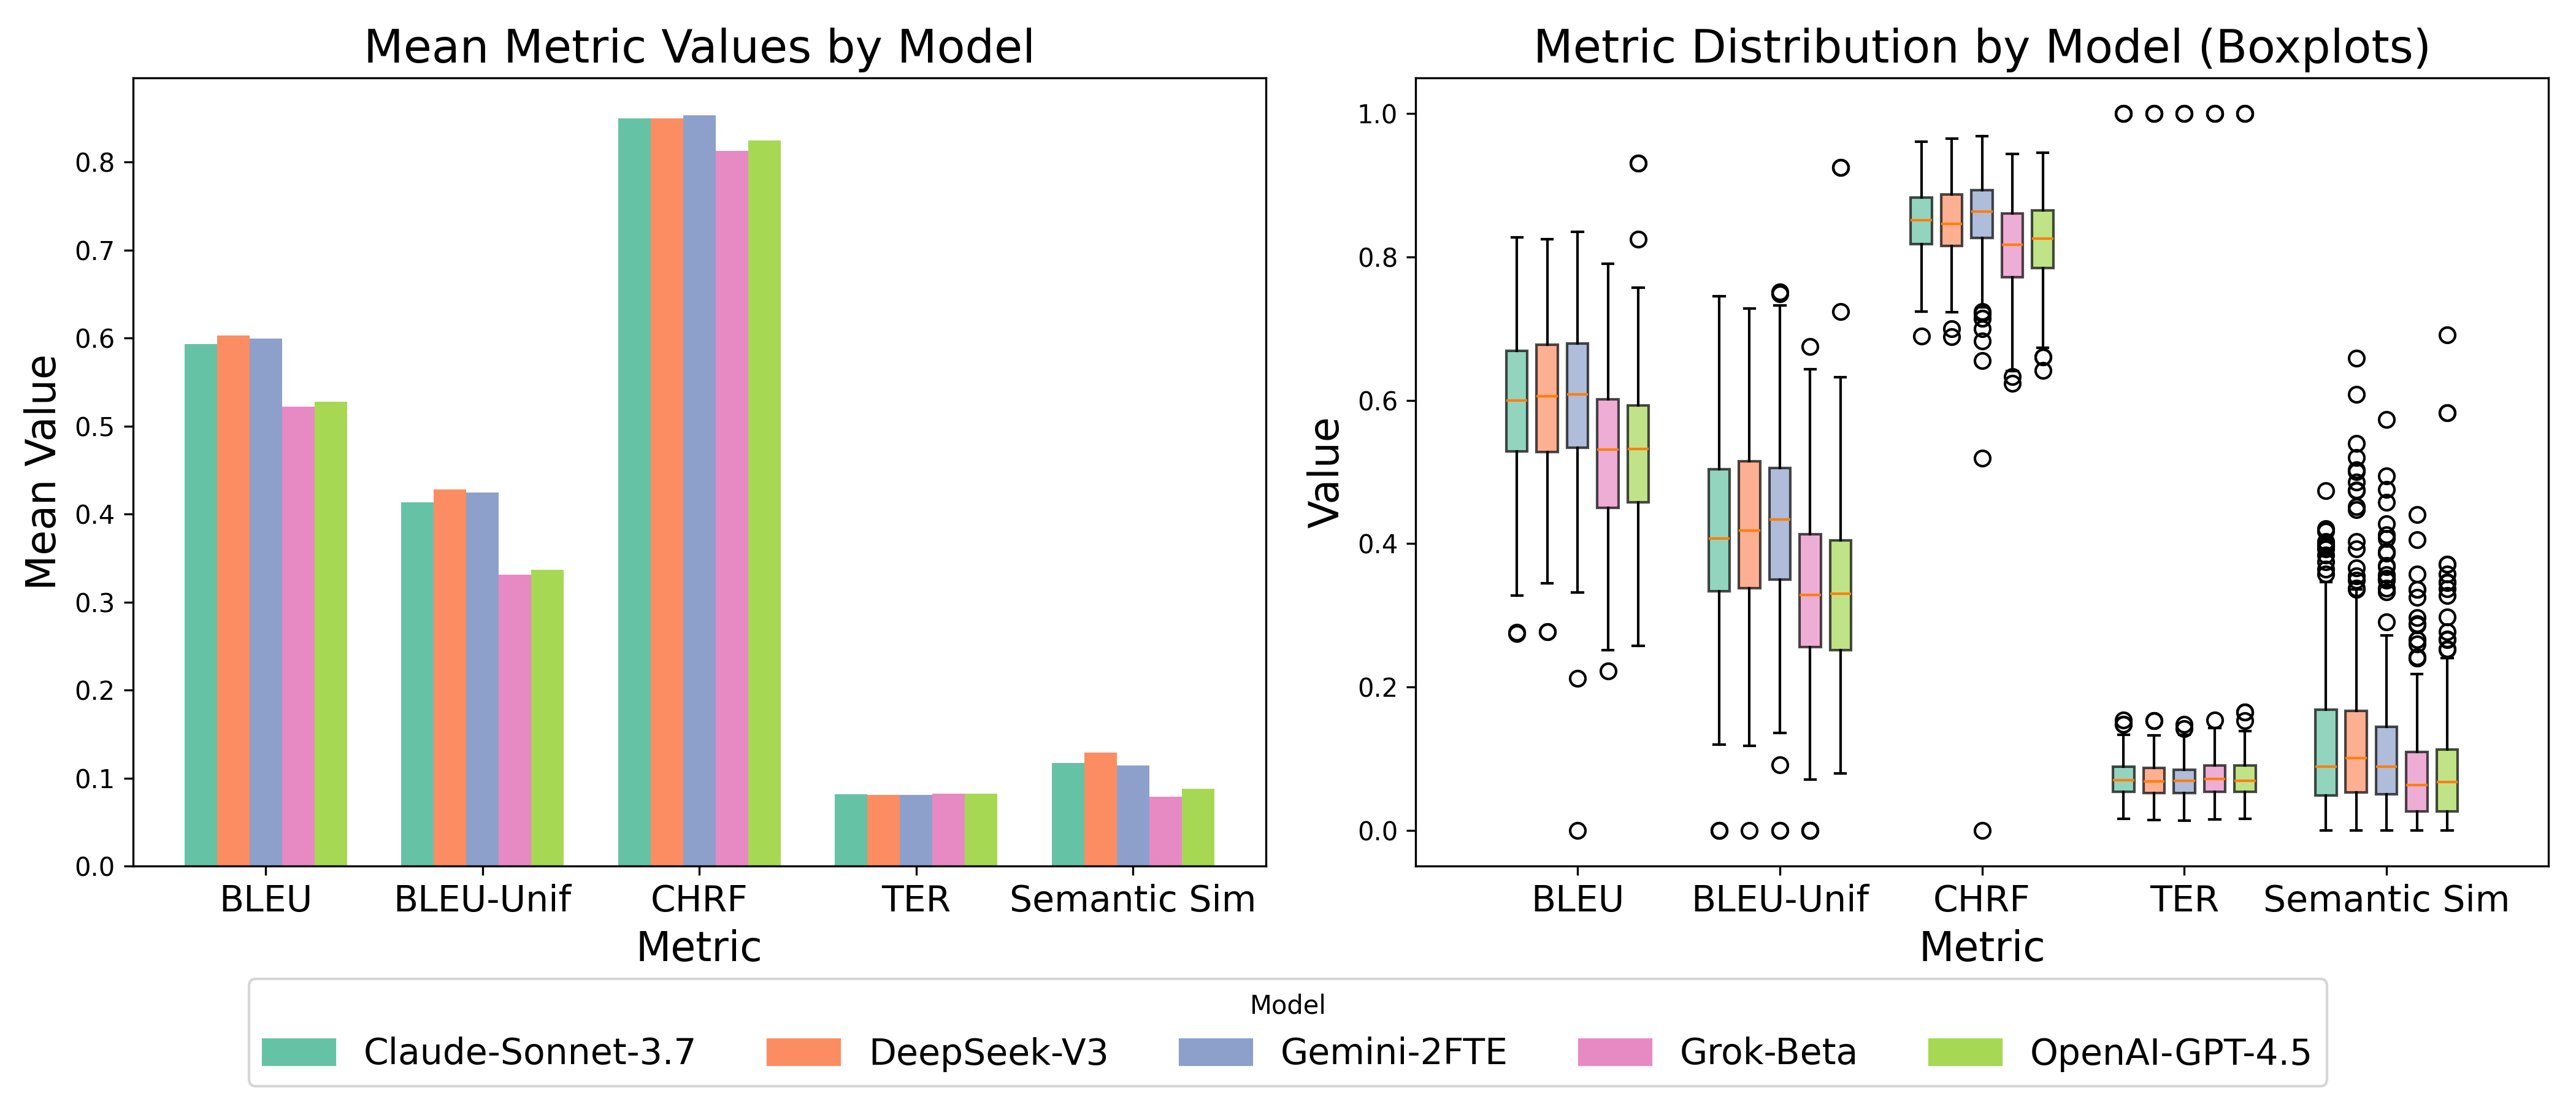
\includegraphics[width=0.8\textwidth]{Figures/metrics_by_model_corrected.png}
    \caption{Comparison of translation metrics across models.}
    \label{fig:metrics_by_model}
\end{figure*}

Translation quality metrics analysis reveals variability among models, with distinct patterns between reasoning-enabled and non-reasoning types. Table~\ref{tab:global_metrics} shows that BLEU averages 0.569 (SD = 0.112), while BLEU-Unif, using uniform weights over 1- to 4-grams, averages 0.386 (SD = 0.133). CHRF, TER and Semantic Similarity report average values of 0.838, 0.082 and 0.105, respectively. This variability, particularly in BLEU-Unif and Semantic Similarity, suggests potential outliers and warrants further investigation into specific model behaviors.

Table~\ref{tab:transposed_model_stats} details the scores by model. Reasoning-enabled models (Claude-Sonnet-3.7, Gemini-2FTE, Grok-Beta) present BLEU means ranging from 0.522 to 0.600 and BLEU-Unif means from 0.331 to 0.425, with CHRF scores between 0.81 and 0.85—indicating consistent surface-level translation quality. Among non-reasoning models, DeepSeek-V3 achieves the highest BLEU (0.603) and BLEU-Unif (0.428), as well as the highest Semantic Similarity (0.129), suggesting strong preservation of meaning. In contrast, OpenAI-GPT-4.5 reports lower BLEU (0.528) and BLEU-Unif (0.336), alongside a reduced Semantic Similarity (0.088), implying reduced semantic alignment despite high maximum BLEU-Unif peaks.

The boxplot analysis (Figure~\ref{fig:metrics_by_model}) reveals the variability in BLEU, BLEU-Unif and Semantic Similarity scores, with outliers in the latter two indicating potential inconsistencies in translation quality. Compact distributions in BLEU, BLEU-Unif and CHRF suggest stable n-gram and character-level overlap, whereas higher dispersion in Semantic Similarity and BLEU-Unif reflects variability in meaning retention and lexical diversity. DeepSeek-V3 and Claude-Sonnet-3.7 exhibit more consistent performance, while OpenAI-GPT-4.5 and Grok-Beta display higher variability, indicating less reliable translation quality across abstracts.

Further examination of Semantic Similarity and BLEU-Unif reveals distinct model behaviors. DeepSeek-V3 achieves the highest means in both metrics but also shows increased dispersion, suggesting occasional semantic lapses or inconsistencies in lexical choices. Claude-Sonnet-3.7 yields similar averages with lower variability, indicating greater stability. Conversely, OpenAI-GPT-4.5 and Grok-Beta register lower scores and broader distributions, potentially due to misinterpretation of domain-specific terminology or artifacts from back-translation strategies. These findings underscore the importance of evaluating both lexical precision and semantic adequacy, especially in scientific abstracts where conceptual fidelity is essential.

In applied scenarios, such differences are particularly relevant for technical domains such as chemistry, where terminological precision and semantic clarity are crucial. Reasoning-enabled models tend to show greater consistency in structural metrics (BLEU, BLEU-Unif and CHRF), but the strong performance of DeepSeek-V3—a non-reasoning model—demonstrates effective semantic preservation, leading all models in BLEU, BLEU-Unif and Semantic Similarity.

Therefore, if semantic retention is prioritized, DeepSeek-V3 may offer practical advantages. In contrast, when structural consistency or domain-specific terminology must be preserved with minimal variation, reasoning-enabled models may provide more stable outputs. Ultimately, the choice of model depends on the trade-off between semantic accuracy and structural reliability for the specific use case.

\subsubsection{Correlation Between Translation Evaluation Metrics and Semantic Similarity}

\begin{figure*}[ht]
    \centering
    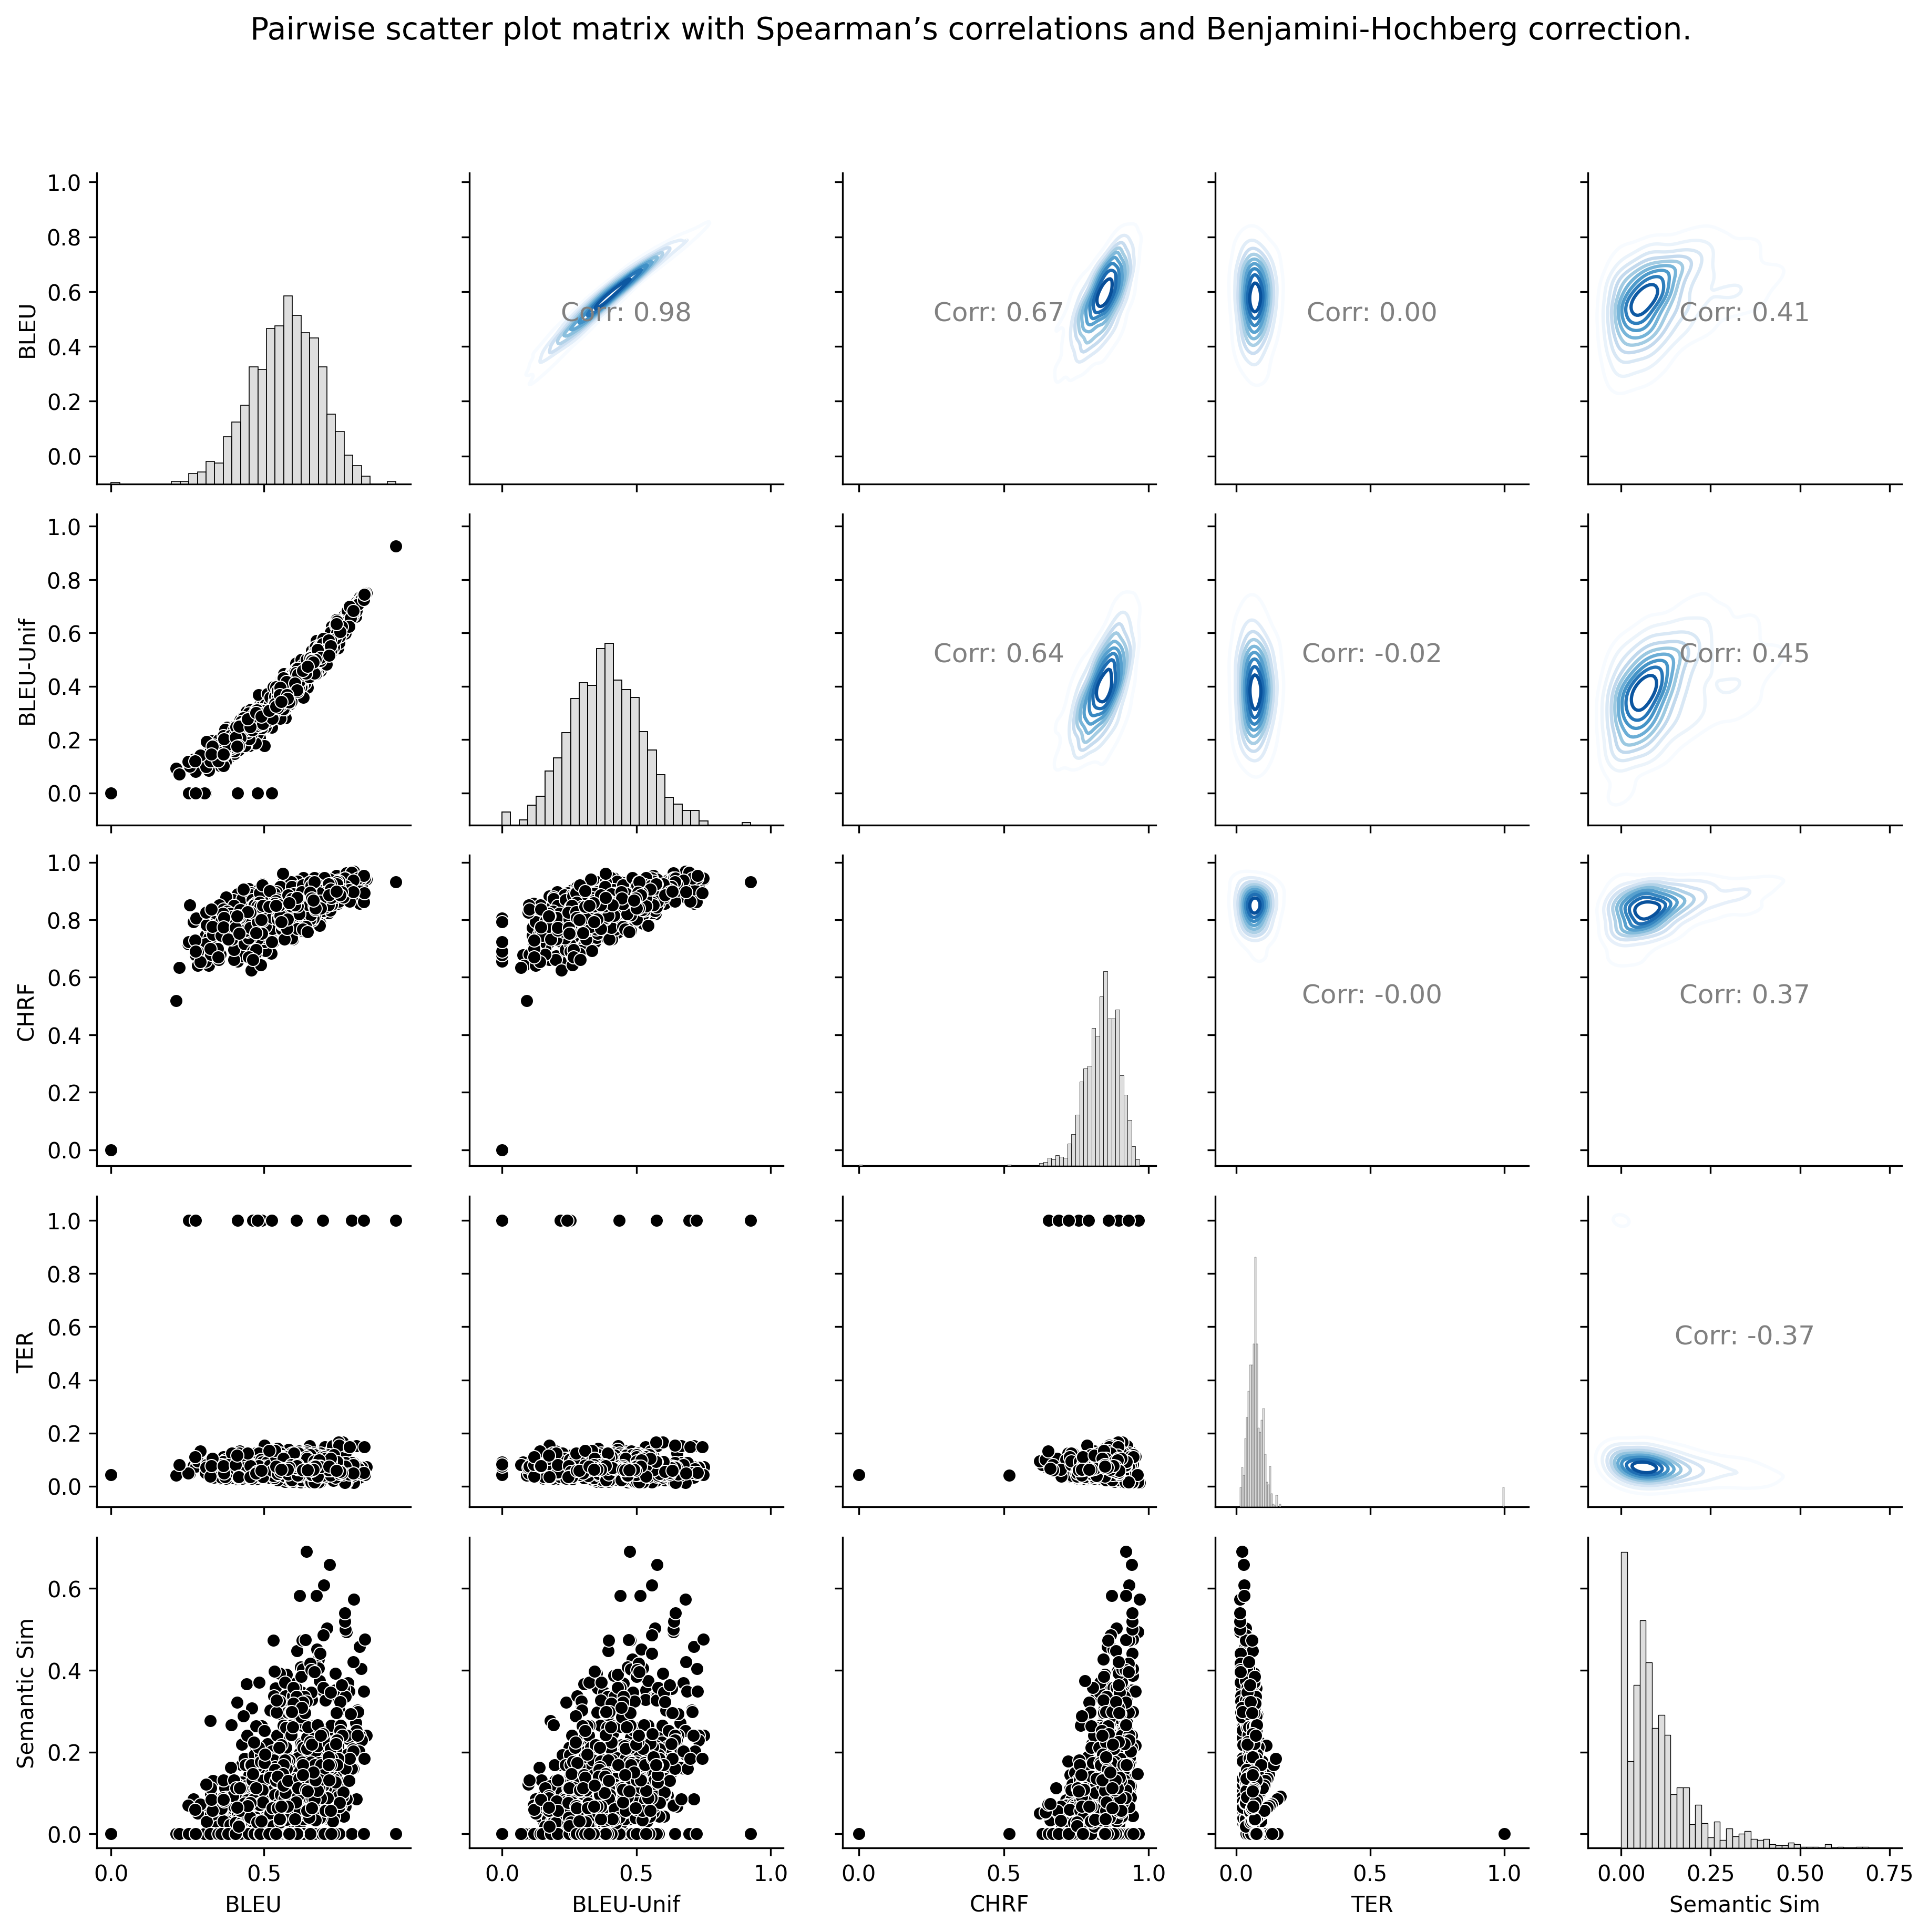
\includegraphics[width=0.8\textwidth]{Figures/pairplot_spearman_correlation_matrix.png}
    \caption{Pairwise scatter plot matrix with Spearman’s correlations and Benjamini-Hochberg correction.}
    \label{fig:metrics_by_model}
\end{figure*}

\begin{figure*}[h]
    \centering
    \begin{minipage}{0.45\textwidth}
        \centering
        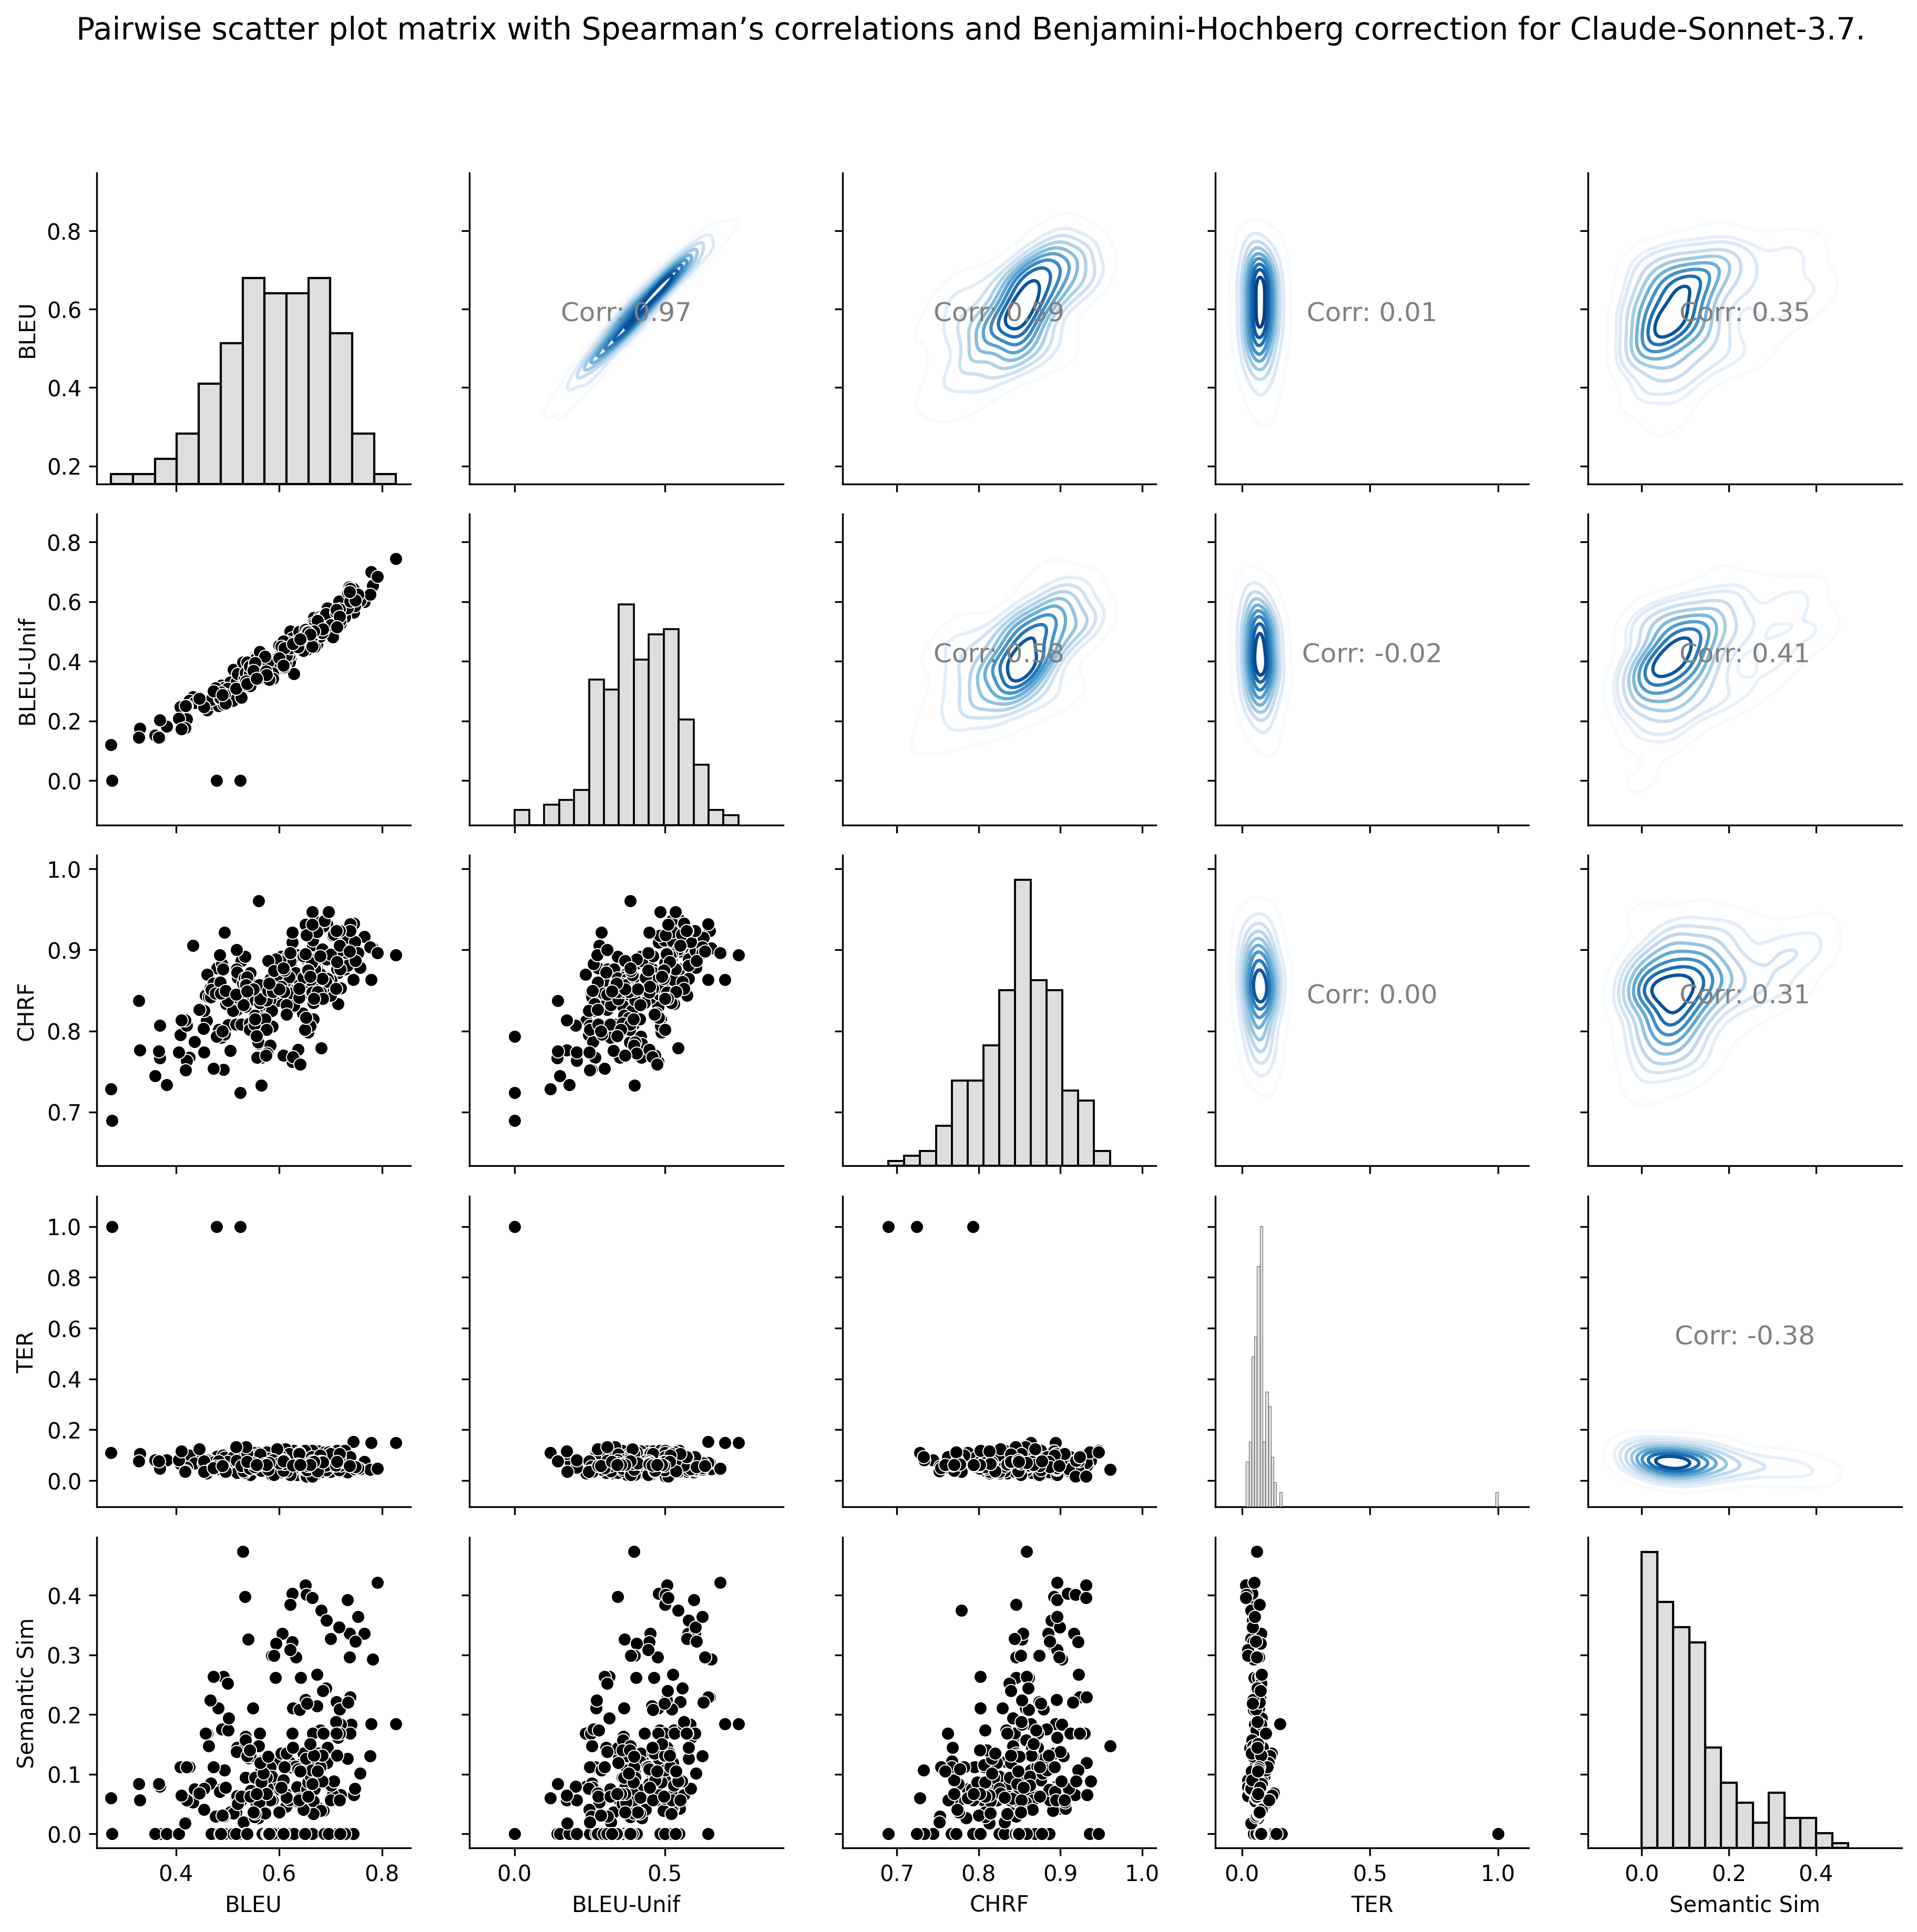
\includegraphics[width=\textwidth]{Figures/pairplot_spearman_correlation_matrix_Claude-Sonnet-3.7.png}
    \end{minipage}
    \hfill
    \begin{minipage}{0.45\textwidth}
        \centering
        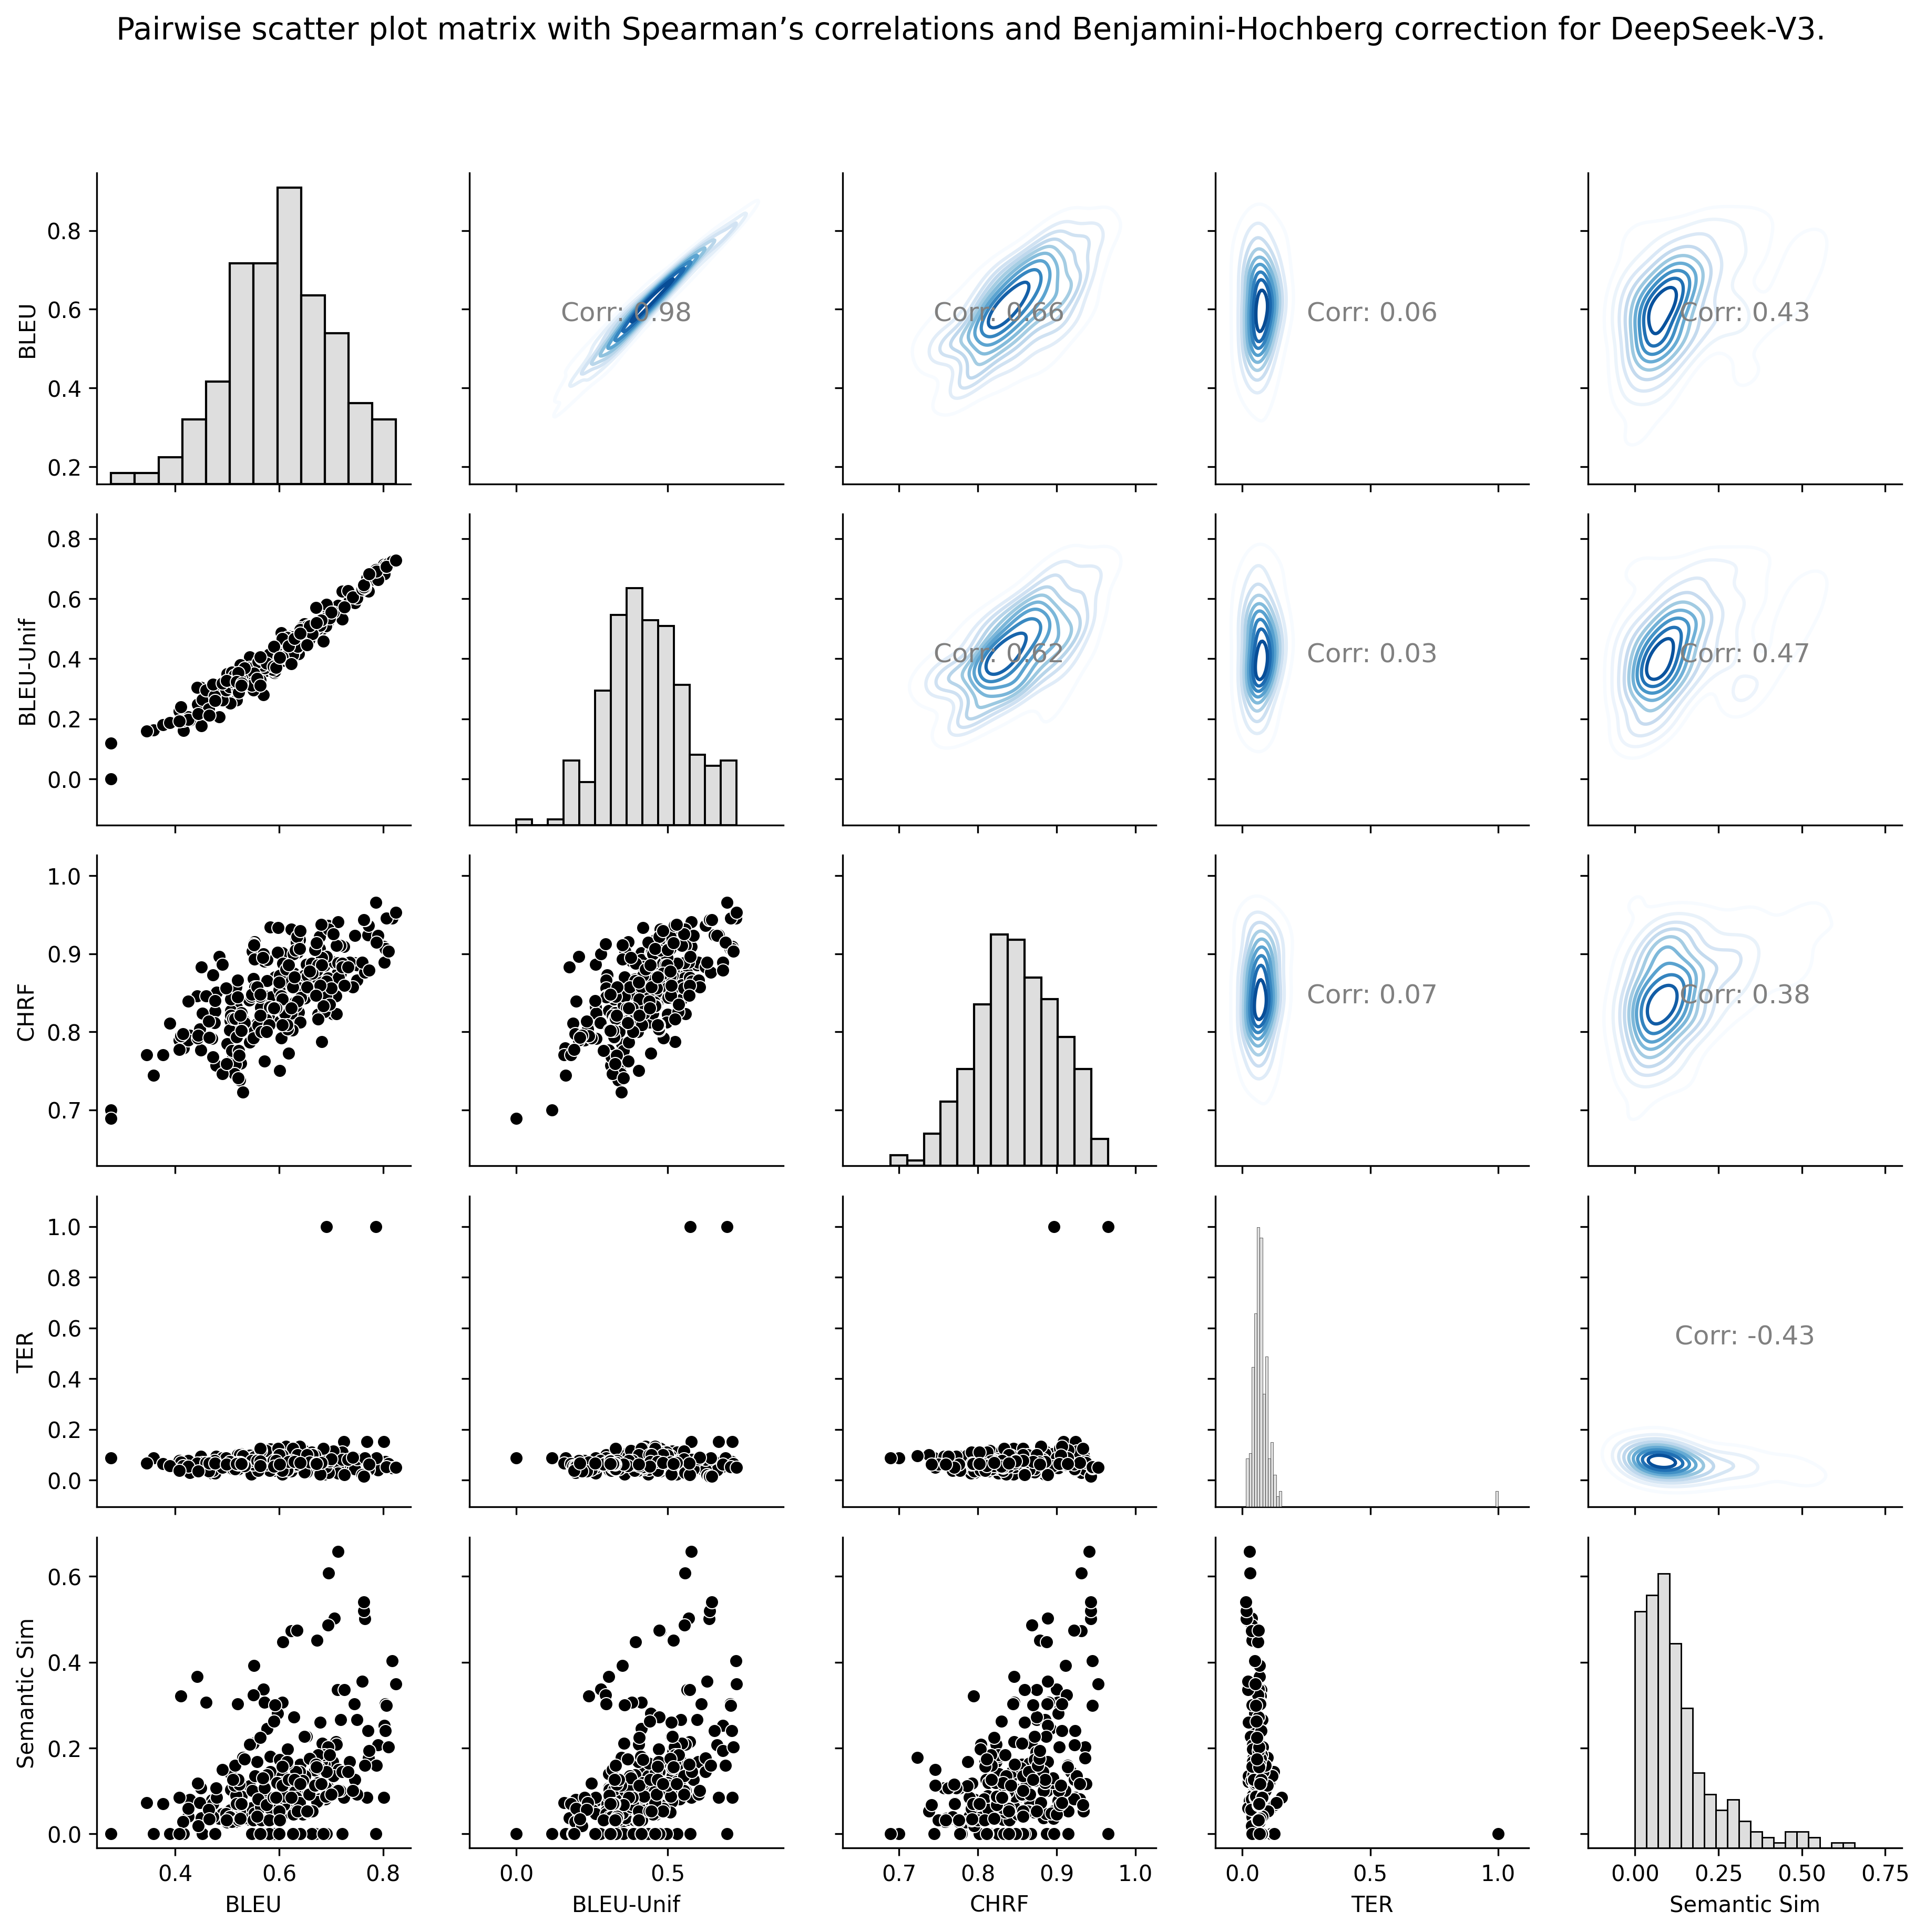
\includegraphics[width=\textwidth]{Figures/pairplot_spearman_correlation_matrix_DeepSeek-V3.png}
    \end{minipage}
    \vspace{0.5cm}
    \begin{minipage}{0.45\textwidth}
        \centering
        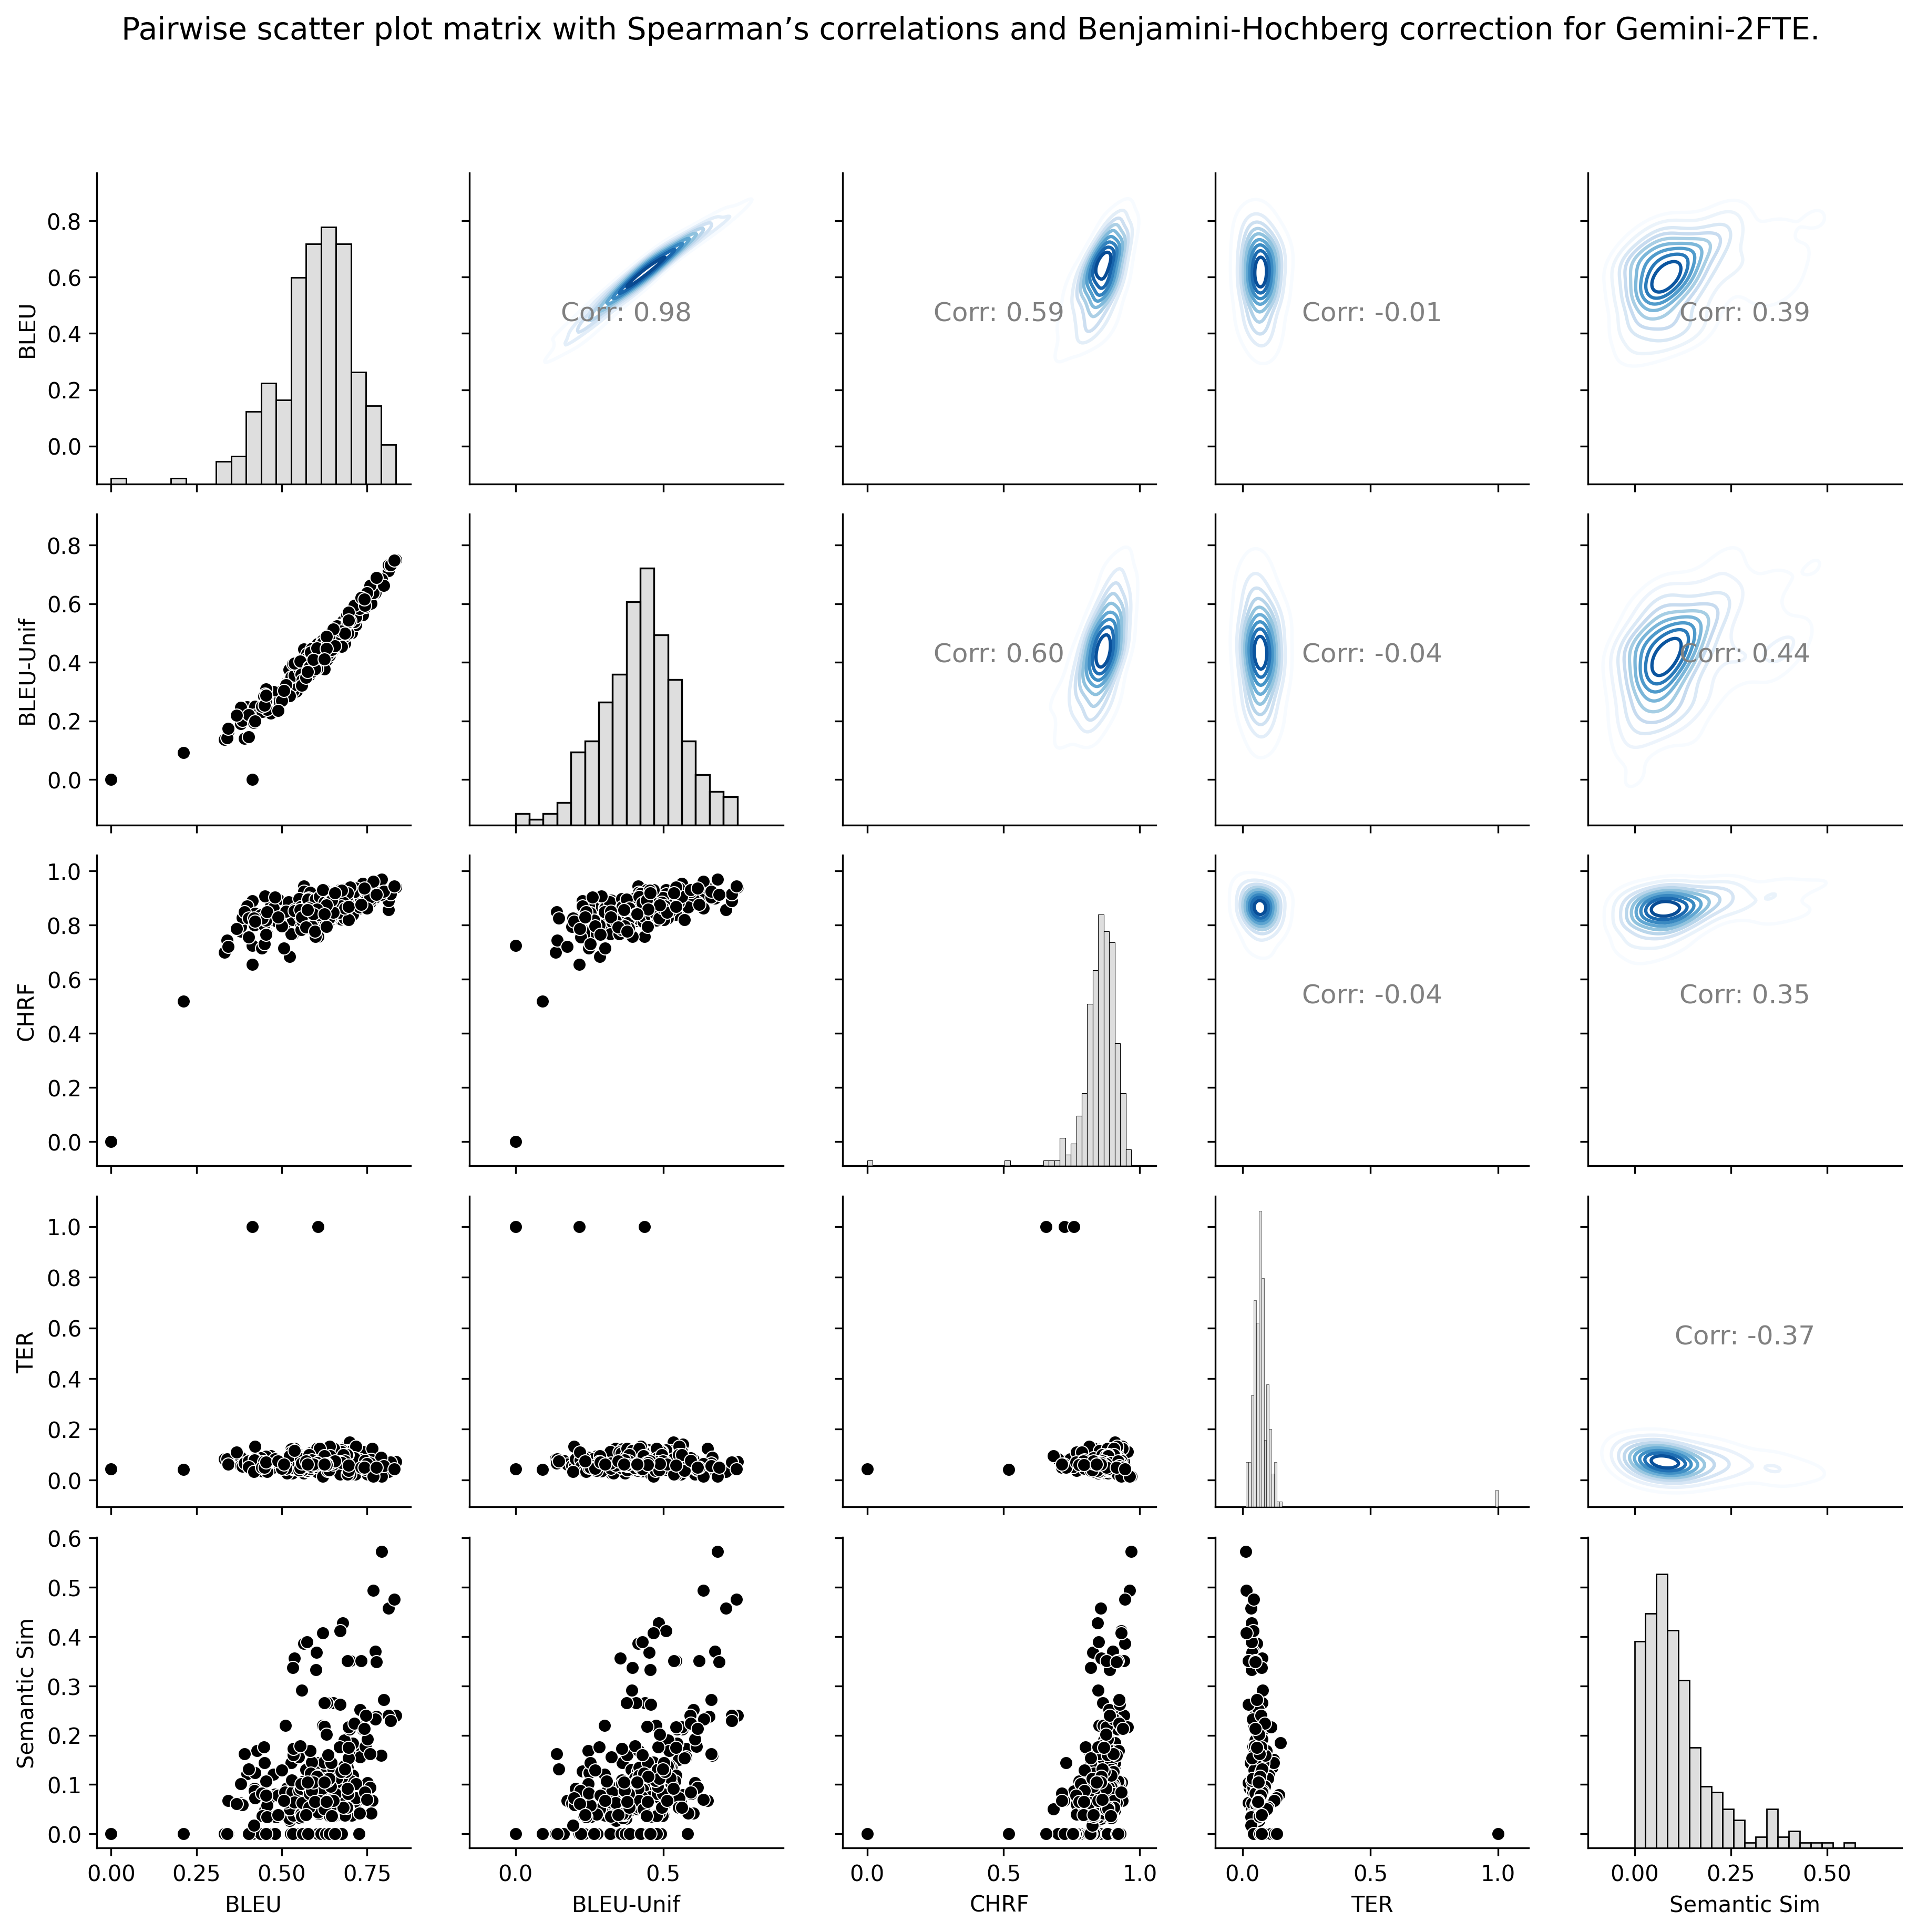
\includegraphics[width=\textwidth]{Figures/pairplot_spearman_correlation_matrix_Gemini-2FTE.png}
    \end{minipage}
    \hfill
    \begin{minipage}{0.45\textwidth}
        \centering
        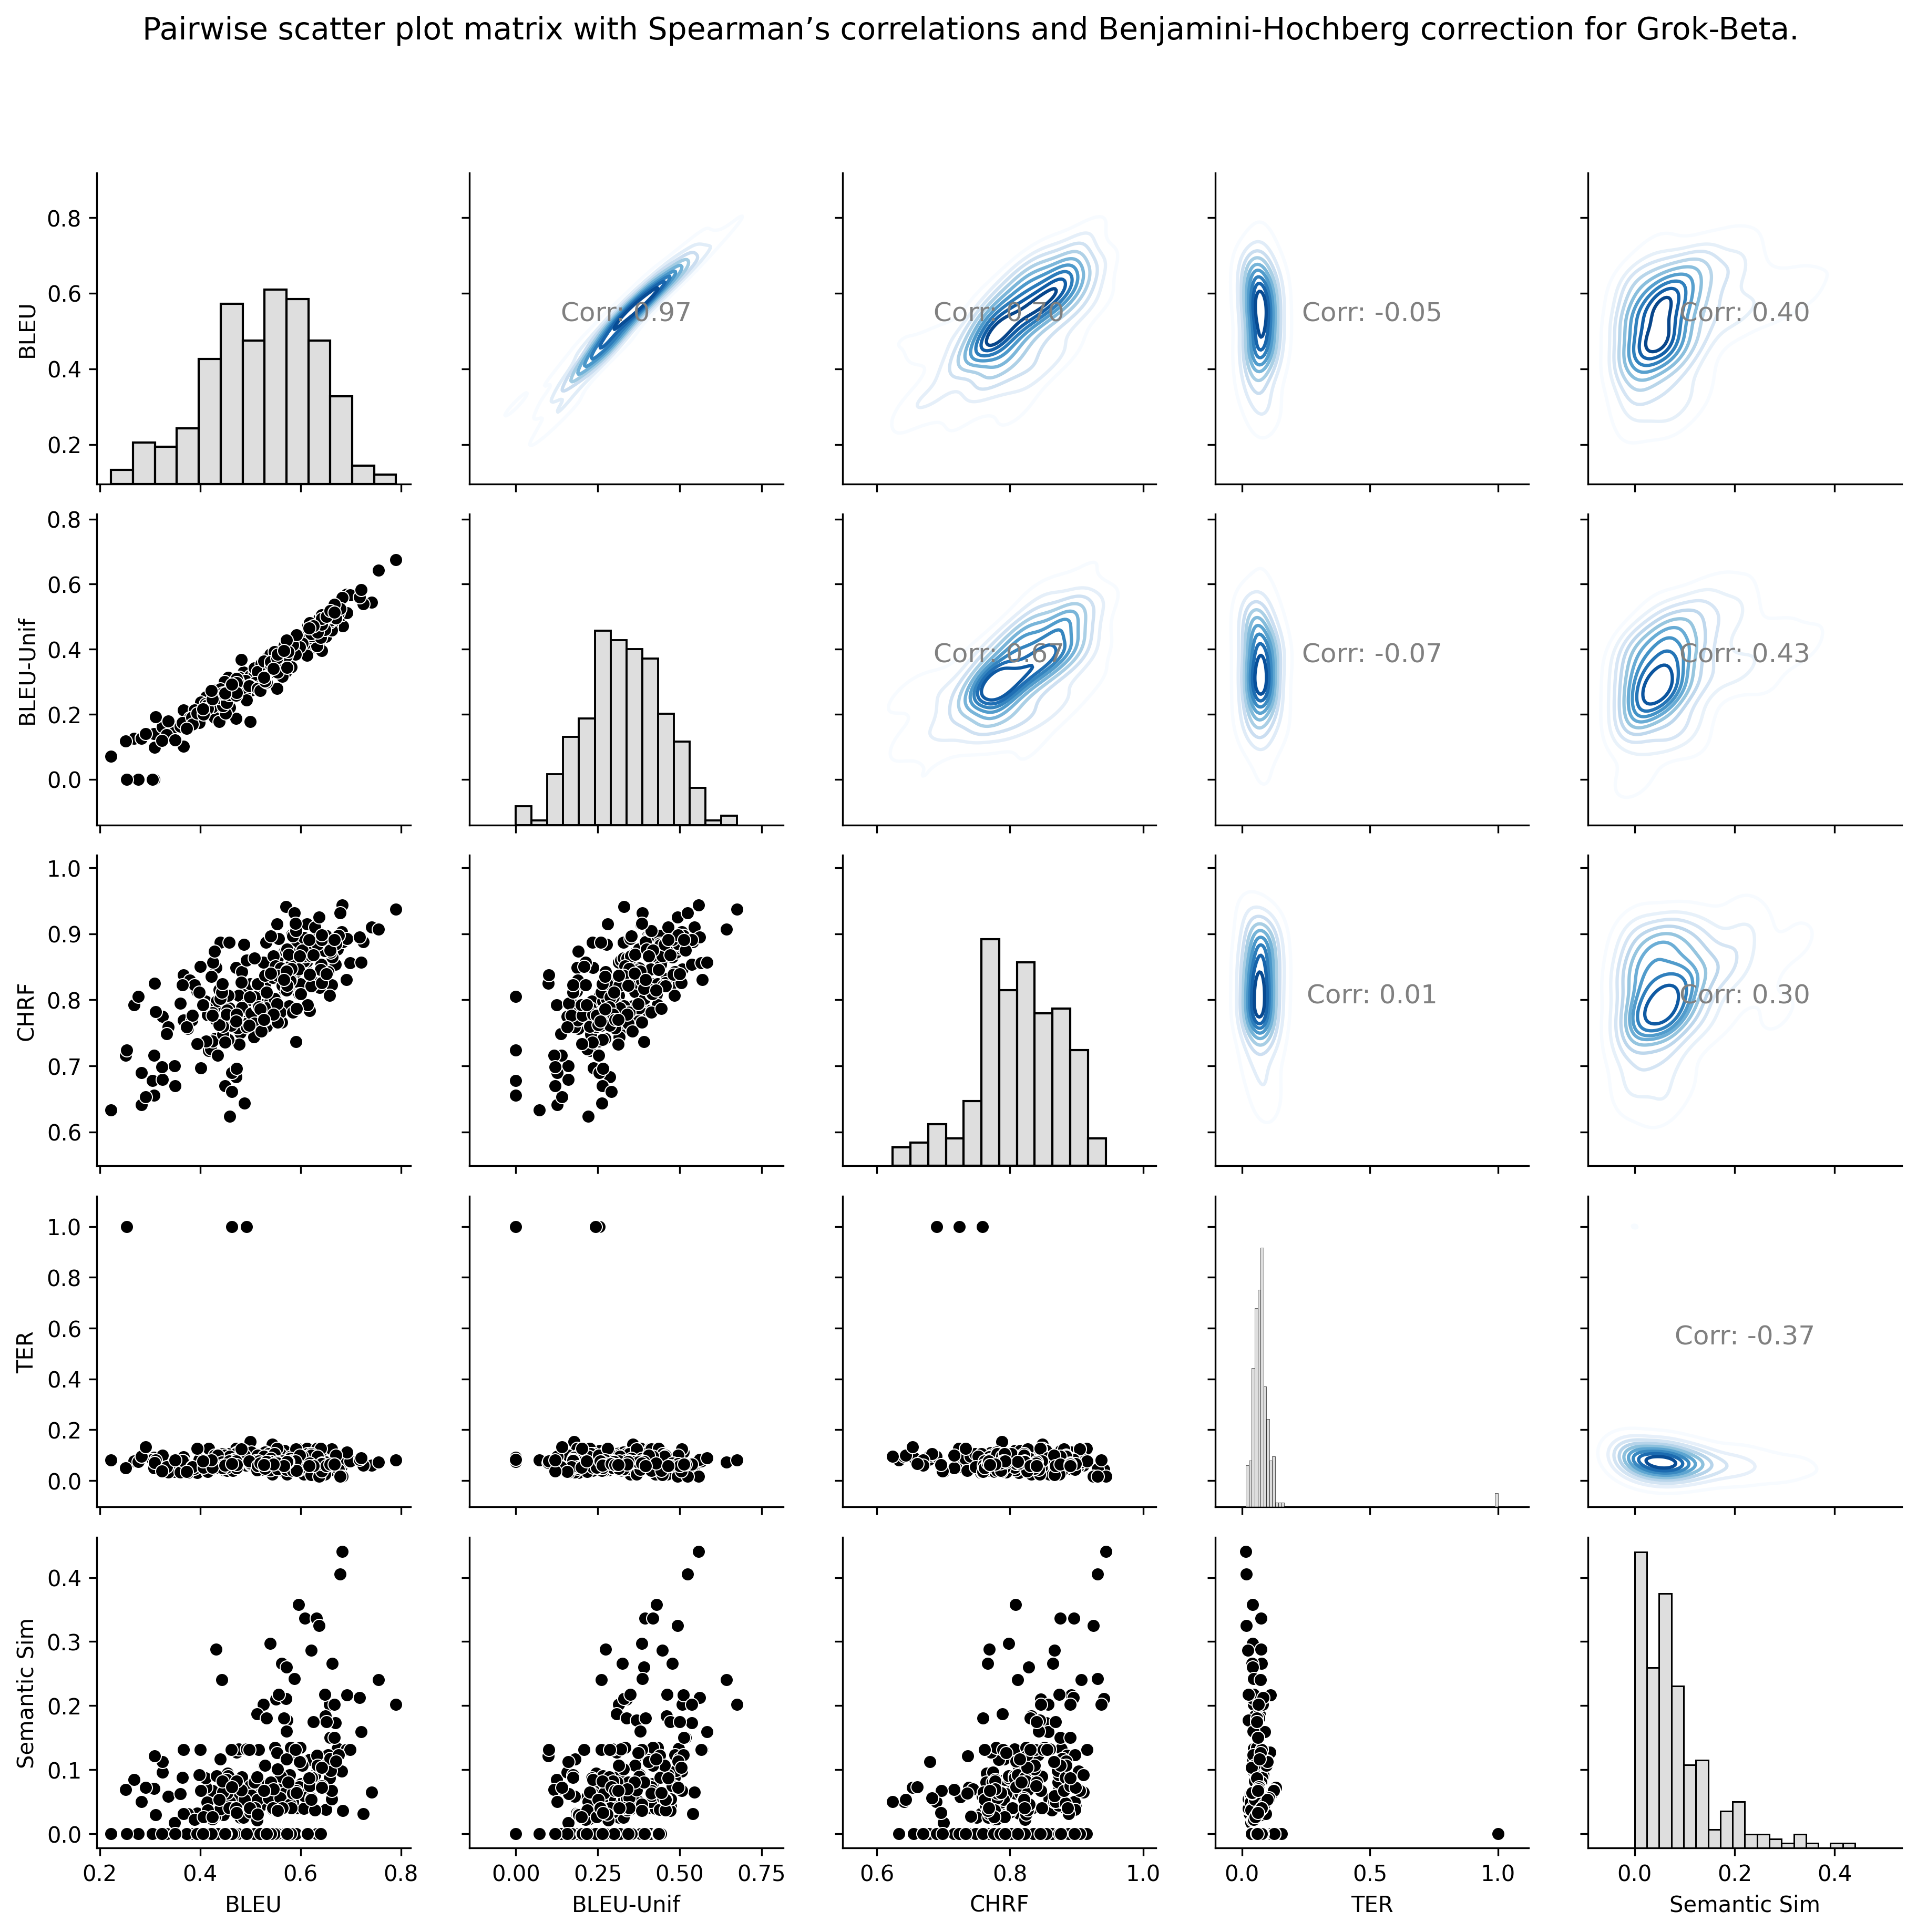
\includegraphics[width=\textwidth]{Figures/pairplot_spearman_correlation_matrix_Grok-Beta.png}
    \end{minipage}
    \vspace{0.5cm}
    \begin{minipage}{0.45\textwidth}
        \centering
        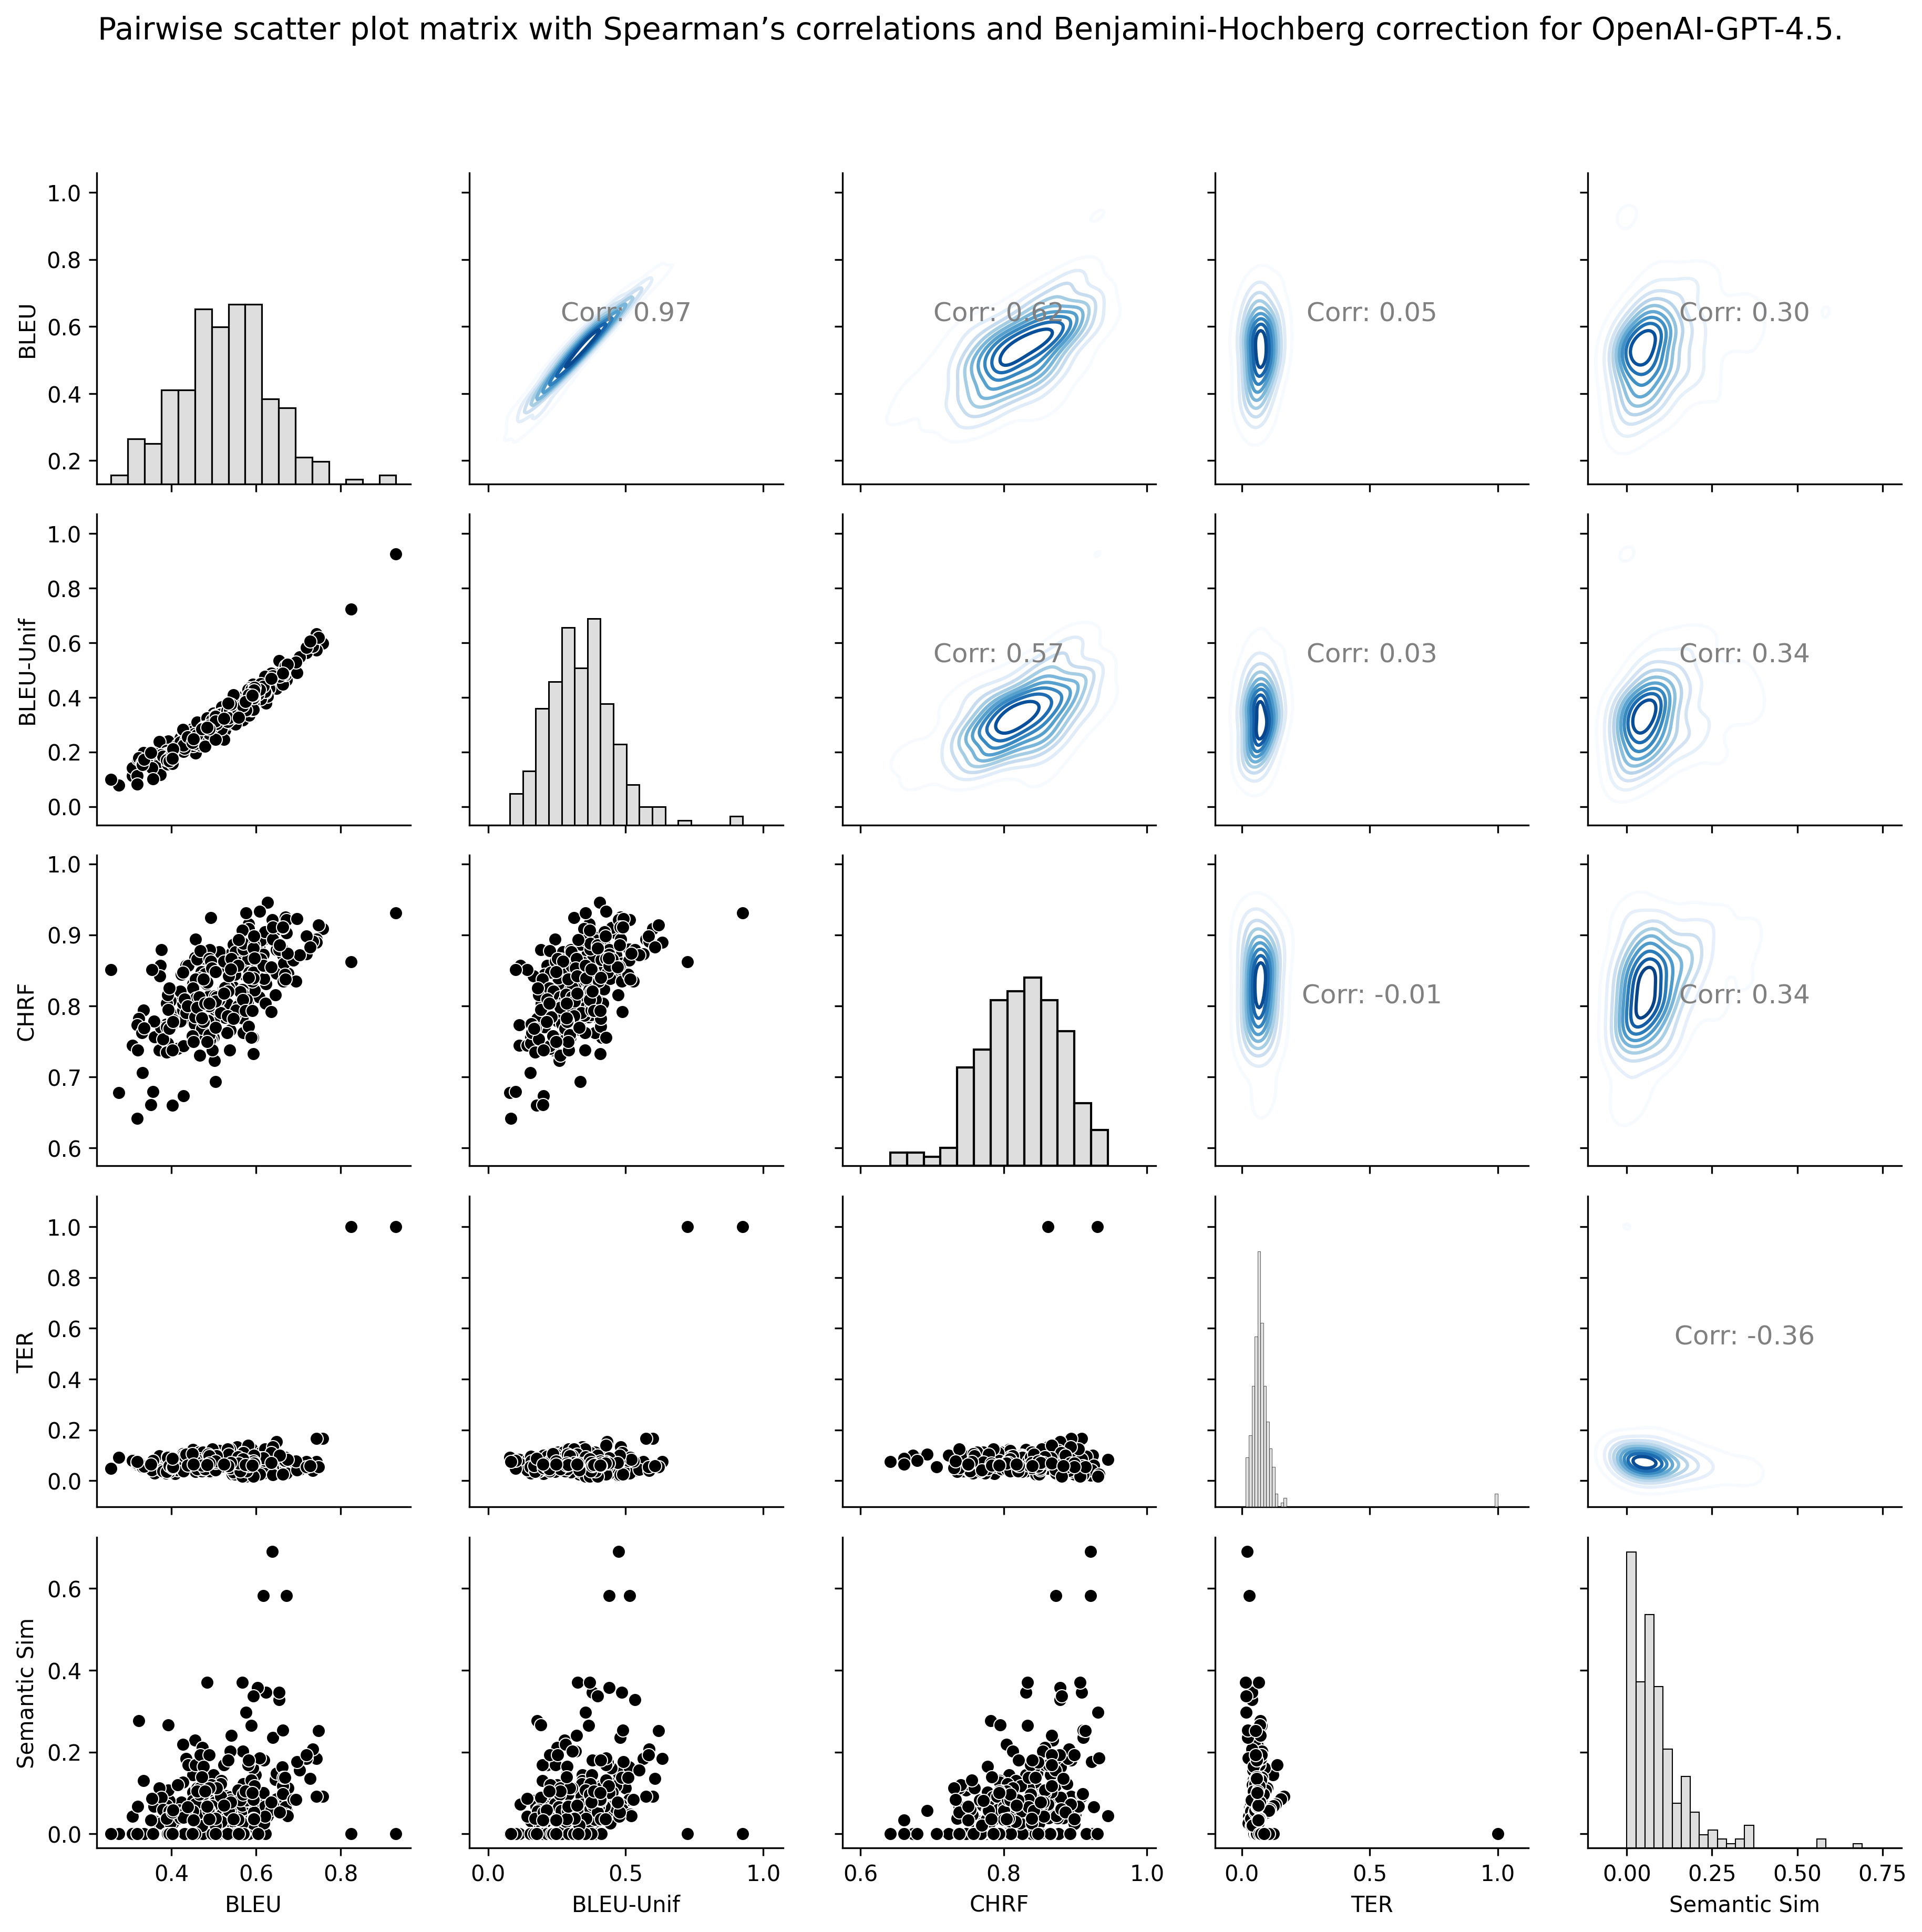
\includegraphics[width=\textwidth]{Figures/pairplot_spearman_correlation_matrix_OpenAI-GPT-4.5.png}
    \end{minipage}
    \caption{Pairwise scatter plot matrices with Spearman's correlations for different models.}
    \label{fig:pairwise_correlation_models}
\end{figure*}

This analysis investigates the relationships among BLEU, BLEU-Unif, CHRF, TER and Semantic Similarity evaluation metrics, both in aggregate (Figure~\ref{fig:metrics_by_model}) and across individual models (Figure~\ref{fig:pairwise_correlation_models}), using Spearman correlation and Benjamini-Hochberg correction.

In the aggregated view, BLEU and CHRF present a correlation of 0.67, suggesting a moderately strong alignment in translation quality estimation. Across individual models, this relationship varies from 0.59 (Claude-Sonnet-3.7, Gemini-2FTE) to 0.70 (Grok-Beta), with Grok-Beta exhibiting the strongest alignment. BLEU-Unif shows consistently high correlation with BLEU across models (above 0.96), confirming that both metrics reflect similar surface-level lexical behavior, though BLEU-Unif incorporates a more balanced n-gram weighting scheme.

BLEU correlates moderately with Semantic Similarity (0.41 overall), with DeepSeek-V3 showing the strongest alignment (0.43), followed closely by Grok-Beta (0.40) and Gemini-2FTE (0.39). BLEU-Unif improves upon this slightly, reaching a higher correlation with Semantic Similarity across all models: 0.47 in DeepSeek-V3, 0.44 in Gemini-2FTE, 0.43 in Grok-Beta, 0.41 in Claude-Sonnet-3.7 and 0.34 in GPT-4.5. These values suggest that BLEU-Unif may be more sensitive to semantic preservation, particularly in models like DeepSeek-V3.

CHRF maintains moderate correlations with Semantic Similarity, ranging from 0.30 (Grok-Beta) to 0.38 (DeepSeek-V3), generally lower than those observed for BLEU-Unif. This indicates that character-level overlap captures some semantic information, but less so than n-gram–based metrics with broader coverage like BLEU-Unif.

In contrast, TER behaves differently. It exhibits a negative overall correlation with Semantic Similarity (-0.37), with DeepSeek-V3 again showing the strongest inverse relationship (-0.43), followed by Claude-Sonnet-3.7 (-0.38) and Grok-Beta (-0.37). These results confirm that greater edit distance implies reduced semantic alignment. Moreover, TER shows near-zero correlation with BLEU (-0.01 to 0.06), BLEU-Unif (-0.04 to 0.03) and CHRF (–0.04 to 0.07), reinforcing its independence as a metric focused on edit operations rather than semantic or lexical similarity.

From a distributional perspective, BLEU, BLEU-Unif and CHRF deviate from normality (Shapiro–Wilk $p < 0.0001$), with BLEU showing slight right-skew, BLEU-Unif exhibiting wider tails and CHRF concentrating near its upper bound. TER values are tightly clustered at low levels, reflecting minimal required corrections. Semantic Similarity is skewed toward the lower end, suggesting that many translations struggle with semantic fidelity. Although the aggregate view provides an overview, the model-wise matrices better expose differences in dispersion, alignment and robustness of each metric.

Overall, DeepSeek-V3 presents the strongest internal coherence, with the highest BLEU-Unif–Semantic Similarity correlation (0.47), confirming its ability to retain meaning consistently. Gemini-2FTE follows closely, combining high BLEU-Unif alignment with moderate CHRF and Semantic Similarity scores. Grok-Beta exhibits the highest BLEU–CHRF correlation (0.70), but more limited semantic fidelity. Claude-Sonnet-3.7 offers balanced but moderate alignment across all metrics, while GPT-4.5 demonstrates the weakest semantic correlation in both BLEU (0.30) and BLEU-Unif (0.34), limiting its suitability in semantically demanding applications.





\subsubsection{Friedman Test and Dunn Post-Hoc Analysis}

The Friedman test, a non-parametric method for paired data, was used to assess differences between translation models based on average metric values. A p-value below 0.05 indicates significant differences, prompting a post-hoc Dunn test for pairwise model comparisons. The Benjamini-Hochberg correction was applied to manage false positives, in contrast to the more conservative Bonferroni method. Additionally, mean differences between statistically distinct model pairs were calculated to quantify the magnitude of those differences. This approach ensures robust and interpretable results, highlighting both the presence and practical relevance of observed differences.

The statistical analysis revealed significant differences across all evaluated metrics—BLEU, BLEU-Unif, CHRF and Semantic Similarity—with the exception of TER, as indicated by Friedman test p-values approaching zero. This confirms that at least one model differs significantly from the others in each metric, except for edit-distance–based performance.

For BLEU, which measures translation fidelity via weighted n-gram overlap, Claude-Sonnet-3.7, DeepSeek-V3 and Gemini-2FTE significantly outperformed Grok-Beta and OpenAI-GPT-4.5, with mean differences ranging from 0.0659 to 0.0810. These findings suggest that the latter models likely perform more reformulations during translation, reducing fidelity to the original text. A similar pattern was observed for BLEU-Unif, which distributes weights uniformly across 1- to 4-grams: the same three models outperformed Grok-Beta and GPT-4.5 with larger mean differences (0.0770 to 0.0972), reinforcing that BLEU-Unif captures additional translation variability. These higher deltas may reflect broader phrase-level divergence, such as that introduced by back-translation strategies.

The CHRF metric, which is sensitive to character-level changes and morphological variation, also showed significant differences between the same groups, though with smaller mean differences (all below 0.05). This suggests that Claude-Sonnet-3.7, DeepSeek-V3 and Gemini-2FTE preserve surface structures more consistently, whereas Grok-Beta and GPT-4.5 tend to introduce morphological variations that slightly reduce CHRF scores without major distortions.

Although the Friedman test indicated significance for TER, Dunn’s post-hoc test revealed no statistically distinguishable pairs. This discrepancy may result from the floor effect caused by low and concentrated TER values, which limits the sensitivity of the post-hoc comparisons. The results imply that despite minor variations, all models require similar levels of post-editing effort to match reference translations.

The Semantic Similarity metric, focused on meaning preservation, also revealed statistically significant differences. Again, Claude-Sonnet-3.7, DeepSeek-V3 and Gemini-2FTE outperformed Grok-Beta and GPT-4.5, with mean differences ranging from 0.0265 to 0.0499. These differences suggest that Grok-Beta and GPT-4.5 may deviate more frequently from the intended meaning, possibly due to hallucinations or overgeneralizations.

Taken together, Claude-Sonnet-3.7, DeepSeek-V3 and Gemini-2FTE emerge as more suitable for high-fidelity translation tasks—such as technical, scientific, or legal documents—where precision and consistency are paramount. Conversely, Grok-Beta and OpenAI-GPT-4.5 may be preferable for creative or literary content, where semantic flexibility and stylistic variation are desirable. Given the absence of significant TER differences, the overall post-editing workload remains comparable across models. Therefore, model selection should be guided by the specific translation context, balancing structural stability, terminological accuracy and semantic preservation.

\begin{table*}[h]
    \centering
    \caption{Summary of Statistical Differences Between Translation Models}
    \begin{tabular}{cc}
        \hline
        \textbf{Metric} & \textbf{Statistically Different Models and Mean Differences} \\
        \hline
        \multirow{6}{*}{BLEU} & Claude-Sonnet-3.7 vs Grok-Beta (0.0712) \\
                              & Claude-Sonnet-3.7 vs OpenAI-GPT-4.5 (0.0659) \\
                              & DeepSeek-V3 vs Grok-Beta (0.0810) \\
                              & DeepSeek-V3 vs OpenAI-GPT-4.5 (0.0757) \\
                              & Gemini-2FTE vs Grok-Beta (0.0774) \\
                              & Gemini-2FTE vs OpenAI-GPT-4.5 (0.0722) \\
        \hline
        \multirow{6}{*}{BLEU-Unif} & Claude-Sonnet-3.7 vs Grok-Beta (0.0823) \\
                                   & Claude-Sonnet-3.7 vs OpenAI-GPT-4.5 (0.0770) \\
                                   & DeepSeek-V3 vs Grok-Beta (0.0972) \\
                                   & DeepSeek-V3 vs OpenAI-GPT-4.5 (0.0919) \\
                                   & Gemini-2FTE vs Grok-Beta (0.0937) \\
                                   & Gemini-2FTE vs OpenAI-GPT-4.5 (0.0884) \\
        \hline
        \multirow{6}{*}{CHRF} & Claude-Sonnet-3.7 vs Grok-Beta (0.0367) \\
                              & Claude-Sonnet-3.7 vs OpenAI-GPT-4.5 (0.0249) \\
                              & DeepSeek-V3 vs Grok-Beta (0.0368) \\
                              & DeepSeek-V3 vs OpenAI-GPT-4.5 (0.0250) \\
                              & Gemini-2FTE vs Grok-Beta (0.0404) \\
                              & Gemini-2FTE vs OpenAI-GPT-4.5 (0.0286) \\
        \hline
        \multirow{6}{*}{Semantic Similarity} & Claude-Sonnet-3.7 vs Grok-Beta (0.0384) \\
                                             & Claude-Sonnet-3.7 vs OpenAI-GPT-4.5 (0.0294) \\
                                             & DeepSeek-V3 vs Grok-Beta (0.0499) \\
                                             & DeepSeek-V3 vs OpenAI-GPT-4.5 (0.0409) \\
                                             & Gemini-2FTE vs Grok-Beta (0.0356) \\
                                             & Gemini-2FTE vs OpenAI-GPT-4.5 (0.0265) \\
        \hline
        TER & No statistically significant differences between pairs \\
        \hline
    \end{tabular}
\end{table*}


\subsubsection{Balancing Fidelity and Fluency - Ranking Translation Models}

Translation model evaluation ranked systems by BLEU, BLEU-Unif, CHRF, TER and Semantic Similarity. DeepSeek-V3 excelled with the highest BLEU (0.6033), BLEU-Unif (0.4283) and Semantic Similarity (0.1287), indicating strong lexical fidelity, balanced n-gram coverage and robust meaning preservation. It also reported one of the lowest TER scores (0.0808), reflecting low post-editing effort. Despite lacking reasoning capabilities, DeepSeek-V3 outperformed all other models, challenging the assumption that reasoning is a prerequisite for high-quality translation.

Gemini-2FTE ranked second, with a competitive BLEU (0.5997) and BLEU-Unif (0.4248) and the highest CHRF score (0.8530), indicating precise character-level alignment. Its TER (0.0808) matched DeepSeek-V3, while Semantic Similarity (0.1144) was slightly lower, suggesting a minor trade-off in semantic retention. Like DeepSeek-V3, Gemini-2FTE achieved top-tier results without relying on explicit reasoning mechanisms, highlighting the potential of non-reasoning models when well-optimized.

Claude-Sonnet-3.7 placed third with BLEU (0.5935), BLEU-Unif (0.4134) and CHRF (0.8494) scores close to the leaders. Its TER (0.0819) was slightly higher, indicating marginally increased editing effort. However, its Semantic Similarity (0.1172) surpassed Gemini-2FTE, reflecting strong meaning preservation. As a reasoning-enabled model, its performance aligns with expectations, though not surpassing the best non-reasoning models.

OpenAI-GPT-4.5 ranked fourth, with lower BLEU (0.5275), BLEU-Unif (0.3364) and CHRF (0.8244) scores, pointing to increased paraphrasing and reduced surface similarity. Its Semantic Similarity (0.0879) was considerably lower, suggesting notable semantic drift. Although TER (0.0824) was comparable to others, its overall translation quality was less consistent. As a reasoning-capable model, GPT-4.5 underperformed relative to non-reasoning models, emphasizing that reasoning alone does not guarantee superior translation.

Grok-Beta ranked last, with the lowest BLEU (0.5223), BLEU-Unif (0.3311) and CHRF (0.8127) scores, indicating poor n-gram and character overlap. It also recorded the highest TER (0.0825) and the lowest Semantic Similarity (0.0788), highlighting considerable meaning loss and suggesting higher post-editing demand. This model appears less suitable for accuracy-sensitive translation tasks.

In summary, DeepSeek-V3 demonstrated that high-quality translation can be achieved without reasoning, leading in BLEU, BLEU-Unif and Semantic Similarity. Claude-Sonnet-3.7 and Gemini-2FTE provided balanced performance, while OpenAI-GPT-4.5 and Grok-Beta lagged in semantic and lexical fidelity. These findings indicate that reasoning is not a prerequisite for translation excellence and that well-designed non-reasoning models can outperform more complex architectures in practical scenarios.




\color{black}


%\begin{table*}[t]
%\centering
%\begin{tabular}{|c|c|c|c|c|c|c|c|c|}
%\hline
%\textbf{Sample ID} & \textbf{Domain} & \textbf{Text Complexity} & \textbf{Reference Translation} & \textbf{Grok xAI} & \textbf{DeepSeek R1} & \textbf{ChatGPT 4.5} & \textbf{Google Translation} & \textbf{Mistral} \\ \hline
%1 & Chemistry & High & Reference 1 & BLEU Score & BLEU Score & BLEU Score & BLEU Score & BLEU Score \\ \hline
%2 & History & Medium & Reference 2 & BLEU Score & BLEU Score & BLEU Score & BLEU Score & BLEU Score \\ \hline
%3 & Literature & Low & Reference 3 & BLEU Score & BLEU Score & BLEU Score & BLEU Score & BLEU Score \\ \hline
%... & ... & ... & ... & ... & ... & ... & ... & ... \\ \hline
%\end{tabular}
%\caption{Extended Experiment Design for Translation Tool Evaluation (Excluding Baidu and Sougo)}
%\label{tab:translation_evaluation_updated}
%\end{table*}

\section{Conclusions}
This study systematically analyzed the linguistic processing effects of pictophonetic and semantic translation (meaning-based translation) and transliteration in the naming of scientific terms through machine translation, particularly using reverse translation experiments with large language models (LLMs). The experimental results demonstrate that meaning-based translation exhibits significantly greater stability and consistency in LLM translation tasks compared to transliteration, while also revealing key challenges in cross-linguistic processing by LLMs.

\begin{itemize}
\item Stability of pictophonetic and semantic translation vs. transliteration. 
\begin{itemize}
\item High consistency of meaning-based translation: The BLEU score for Chinese chemical element names translated using meaning-based strategies reached 1.00 in reverse translation tasks, indicating high linguistic consistency with virtually no information loss. For instance, "氢" → "Hydrogen" (DeepSeek) → "氢" (GPT-4) retained its original meaning completely.
\item Significant variation in transliteration: The BLEU scores for transliterated heterocyclic compound names were notably lower (0.55–0.65), with substantial variations in back-translations. For example, "千里光碱类" → "Senecionines" (DeepSeek) → "千里光宁类" (Gemini) reflects the inherent irreversibility of transliteration in LLM processing, which is significantly affected by phonetic variations and spelling mappings.
\item Empirical support for meaning-based translation: These results quantitatively validate the long-standing consensus that meaning-based translation is superior to transliteration in scientific term naming, providing new empirical evidence for cross-linguistic terminology strategies.
\end{itemize}
\item Limitations of LLMs in Translation Tasks.
\begin{itemize}
\item Verbatim back-translation: LLMs often exhibit a "back-translation" phenomenon, where they output near-identical versions of the original text, leading to artificially high BLEU scores (e.g., DeepSeek scored 0.996), which may compromise translation evaluation reliability.
\item Task refusal: Gemini refused to process the ZH100 dataset due to computational overload, highlighting differences in task execution capabilities and optimization strategies among different LLMs. This suggests the need for better task scheduling and load balancing in future LLM development.
\item Variation in translation quality across LLMs: The BLEU scores for reverse translations varied across DeepSeek, GPT-4 and Gemini, indicating that differences in translation strategies and training data significantly impact translation quality.
\end{itemize}
\item Implications for NLP and Machine Translation.
\begin{itemize}
\item Impact on Chinese NLP: This study confirms the stability of meaning-based translation in NLP tasks, suggesting that Chinese language standardization efforts should prioritize meaning-based strategies to enhance machine processability and translation consistency.
\item Impact on LLM-based machine translation: Transliteration exhibited high translation variability, suggesting that current LLMs struggle with the accurate back-translation of transliterated terms. Future improvements may involve multimodal language modeling or joint phoneme-semantic training to enhance the consistency of transliterated term translations.
\item Impact on scientific terminology naming: This study introduces a quantitative BLEU evaluation method, which can be applied to optimize terminology naming in various scientific domains, contributing to the standardization of scientific language.
\end{itemize}
\item Innovations in Research Methodology.
\begin{itemize}
    \item Multi-LLM experimental design: By using multiple LLMs, this study minimized model bias, improving the reliability of translation evaluations.
    \item Expanded dataset coverage: The study incorporated nearly 300 term samples across multiple specialized fields, including chemistry, biology and computer science, to verify cross-domain translation patterns.
    \item BLEU-based quantitative analysis framework: This study proposed a reproducible BLEU evaluation framework for automatic assessment of cross-linguistic terminology translation.
    \item Potential for broader applications: The proposed method can be further extended to other language pairs (e.g., English-French, Japanese-Korean) or cross-modal translation tasks (e.g., text-to-speech conversion).
\end{itemize}
\item Future Research Directions. While this study provides an initial investigation into LLM processing of meaning-based and transliterated scientific terms, several areas warrant further exploration:
\begin{itemize}
\item  Integration of human evaluation: Future research should incorporate linguists and professional translators to complement BLEU-based assessments and provide a more comprehensive analysis of translation quality.
\item  Optimization of LLM translation performance: Further studies should explore ways to enhance LLMs’ handling of transliteration tasks, such as incorporating phoneme-based information or speech-assisted models to improve cross-linguistic consistency.
\end{itemize}

This study demonstrates that meaning-based translation is significantly more stable and reliable than transliteration in LLM processing, while also identifying key limitations of LLMs in terminology translation. The findings provide new quantitative evidence and research insights for Chinese NLP, scientific terminology standardization and LLM translation optimization. Future research can extend these findings to multilingual and multimodal translation tasks, contributing to the broader advancement of machine translation and language processing.

\color{blue}
The findings of this study provide empirical support for prioritizing semantic translation strategies in the standardization of scientific nomenclatures, particularly for ideographic languages such as Chinese. Additionally, the results suggest that traditional metrics like BLEU can be complemented by computational cost analyses to optimize the implementation of LLMs in technical and scientific translation tasks. Future research may explore hybrid approaches that combine semantic and phonetic translation to enhance meaning preservation in highly specialized terms.
\color{black}

\end{itemize}

% The preferred spelling of the word ``acknowledgment'' in America is without 
% an ``e'' after the ``g''. Avoid the stilted expression ``one of us (R. B. 
% G.) thanks $\ldots$''. Instead, try ``R. B. G. thanks$\ldots$''. Put sponsor 
% acknowledgments in the unnumbered footnote on the first page.

% \section*{References}

% Please number citations consecutively within brackets \cite{b1}. The 
% sentence punctuation follows the bracket \cite{b2}. Refer simply to the reference 
% number, as in \cite{b3}---do not use ``Ref. \cite{b3}'' or ``reference \cite{b3}'' except at 
% the beginning of a sentence: ``Reference \cite{b3} was the first $\ldots$''

% Number footnotes separately in superscripts. Place the actual footnote at 
% the bottom of the column in which it was cited. Do not put footnotes in the 
% abstract or reference list. Use letters for table footnotes.

% Unless there are six authors or more give all authors' names; do not use 
% ``et al.''. Papers that have not been published, even if they have been 
% submitted for publication, should be cited as ``unpublished'' \cite{b4}. Papers 
% that have been accepted for publication should be cited as ``in press'' \cite{b5}. 
% Capitalize only the first word in a paper title, except for proper nouns and 
% element symbols.

% For papers published in translation journals, please give the English 
% citation first, followed by the original foreign-language citation \cite{b6}.

% \begin{thebibliography}{00}
% \bibitem{b1} G. Eason, B. Noble and I. N. Sneddon, ``On certain integrals of Lipschitz-Hankel type involving products of Bessel functions,'' Phil. Trans. Roy. Soc. London, vol. A247, pp. 529--551, April 1955.
% \bibitem{b2} J. Clerk Maxwell, A Treatise on Electricity and Magnetism, 3rd ed., vol. 2. Oxford: Clarendon, 1892, pp.68--73.
% \bibitem{b3} I. S. Jacobs and C. P. Bean, ``Fine particles, thin films and exchange anisotropy,'' in Magnetism, vol. III, G. T. Rado and H. Suhl, Eds. New York: Academic, 1963, pp. 271--350.
% \bibitem{b4} K. Elissa, ``Title of paper if known,'' unpublished.
% \bibitem{b5} R. Nicole, ``Title of paper with only first word capitalized,'' J. Name Stand. Abbrev., in press.
% \bibitem{b6} Y. Yorozu, M. Hirano, K. Oka and Y. Tagawa, ``Electron spectroscopy studies on magneto-optical media and plastic substrate interface,'' IEEE Transl. J. Magn. Japan, vol. 2, pp. 740--741, August 1987 [Digests 9th Annual Conf. Magnetics Japan, p. 301, 1982].
% \bibitem{b7} M. Young, The Technical Writer's Handbook. Mill Valley, CA: University Science, 1989.
% \end{thebibliography}
% \vspace{12pt}

% \section*{ACKNOWLEDGMENT}

% This work has been partially supported by the Brazilian National Council for Scientific and Technological Development (CNPq) under the grant number 309545/2021-8.



%%%%%%%%%%%%%%%%%%%%%%%%%%%%%%%%%%%%%%%%%%%%%%%%%%%%%%%%%%%%%%%%%%%%%%%%%%%%%%%%
\section*{ACKNOWLEDGMENT}
We sincerely appreciate the public translation and text refinement services provided by ChatGPT, Grok, DeepSeek, QwenVL, Gemini, Mistral, Google Translate, Baidu Translate and Sogou Translate, which played a crucial role in the cross-linguistic processing and analysis conducted in this study.

\bibliographystyle{IEEEtran}
\bibliography{IEEEabrv,Ref.bib}
\end{CJK*}

\end{document}
